% !TeX document-id = {55cdd1f2-c708-43a6-9dcf-ca7bc9e91f17}
% !BIB program = biber
\documentclass[10pt]{beamer}

\usetheme{scilifelab}
\usepackage{appendixnumberbeamer}

\usepackage{booktabs}
\usepackage[scale=2]{ccicons}

\usepackage{hyperref}
\hypersetup{colorlinks=true, linkcolor=scAqua, urlcolor=scAqua, citecolor=scAqua}

\usepackage[backend=biber,style=apa, sortcites=true,sorting=nyt]{biblatex}
\addbibresource{literature/base-odyssey.bib}

\usepackage[savemem]{listings}
\lstset{
	basicstyle=\footnotesize\ttfamily\fontfamily{lmtt}\selectfont,          % Font style
	xleftmargin=-30pt,               % Remove left margin (adjust as needed)
	xrightmargin=0pt,              % Remove right margin (optional)
	breaklines=true,               % Allows line breaks in long lines of code
	captionpos=b                   % Position of the caption (if any)
	aboveskip=0pt,                 % Space before the listing
	belowskip=0pt,                 % Space after the listing
	framexleftmargin=-50pt,         % Padding inside the left frame
	framexrightmargin=0pt,        % Padding inside the right frame
	framesep=0pt,              
}
\renewcommand{\ttdefault}{lmtt}


\usepackage{pgfplots}
\usepgfplotslibrary{dateplot}

\usepackage{xspace}
\newcommand{\themename}{\textbf{\textsc{scilifelab}}\xspace}
\newcommand{\credit}[1]{{\vskip0pt plus 1filll \par \raggedleft \scriptsize \mdseries \color{mDarkBrown} #1 \par}}
\newcommand{\creditdark}[1]{{\vskip0pt plus 1filll \par \raggedleft \scriptsize \mdseries \color{scMGray} #1 \par}}
\newcommand{\creditdarknofill}[1]{{\par \raggedleft \scriptsize \mdseries \color{scMGray} #1 \par}}
\newcommand{\creditleft}[1]{{\vskip0pt plus 1filll \par \raggedright \scriptsize \mdseries \color{mDarkBrown} #1 \par}}
\newcommand{\creditdarkleft}[1]{{\vskip0pt plus 1filll \par \raggedright \scriptsize \mdseries \color{scMGray} #1 \par}}
\newcommand{\creditdarkleftnofill}[1]{{\par \raggedright \scriptsize \mdseries \color{scMGray} #1 \par}}
\newcommand{\citeme}[1]{{\xspace\color{scAqua} \scriptsize [\cite{#1}]}}
\newcommand{\feature}[1]{{\color{scLime} \textbf{#1}}}
\newcommand{\remark}[1]{{\par \color{scGrape} \ensuremath{\rightarrow} \emph{#1}}}

\makeatletter
\newcommand*{\myroman}[1]{{\fontfamily{ptm}\selectfont \expandafter\@slowromancap\romannumeral #1@}}
\makeatother

\title{2001: A Base Odyssey}
\subtitle{The era of genomics and massive parallel sequencing}
\date{February 24, 2025}
\author{Matthias Zepper, PhD}
\institute{NGI Stockholm\par \href{https://ngisweden.scilifelab.se}{https://ngisweden.scilifelab.se}}
\titlegraphic{\hfill
\includegraphics[height=1cm]{./additional_graphics/SciLifeLab_Logotype_Green_POS.png}}

\begin{document}

\maketitle

\begin{frame}{2001: Draft assemblies of the human genome are published}
	\begin{figure}
		
\includegraphics[width=0.8\textwidth]{figures/humangenomeproject.png}
		\caption{The private company Celera\citeme{Venter2001} and the International Human Genome Sequencing Consortium\citeme{Lander2001} both publish a draft sequence of the euchromatic portion of the human genome.}
	\end{figure}
	\credit{doi: 10.1126/science.1058040; doi: 10.1038/35057062}
\end{frame}

\begin{frame}[standout]{The overture to the genomic era}
	\begin{figure}
		\hspace*{-1.1cm}
		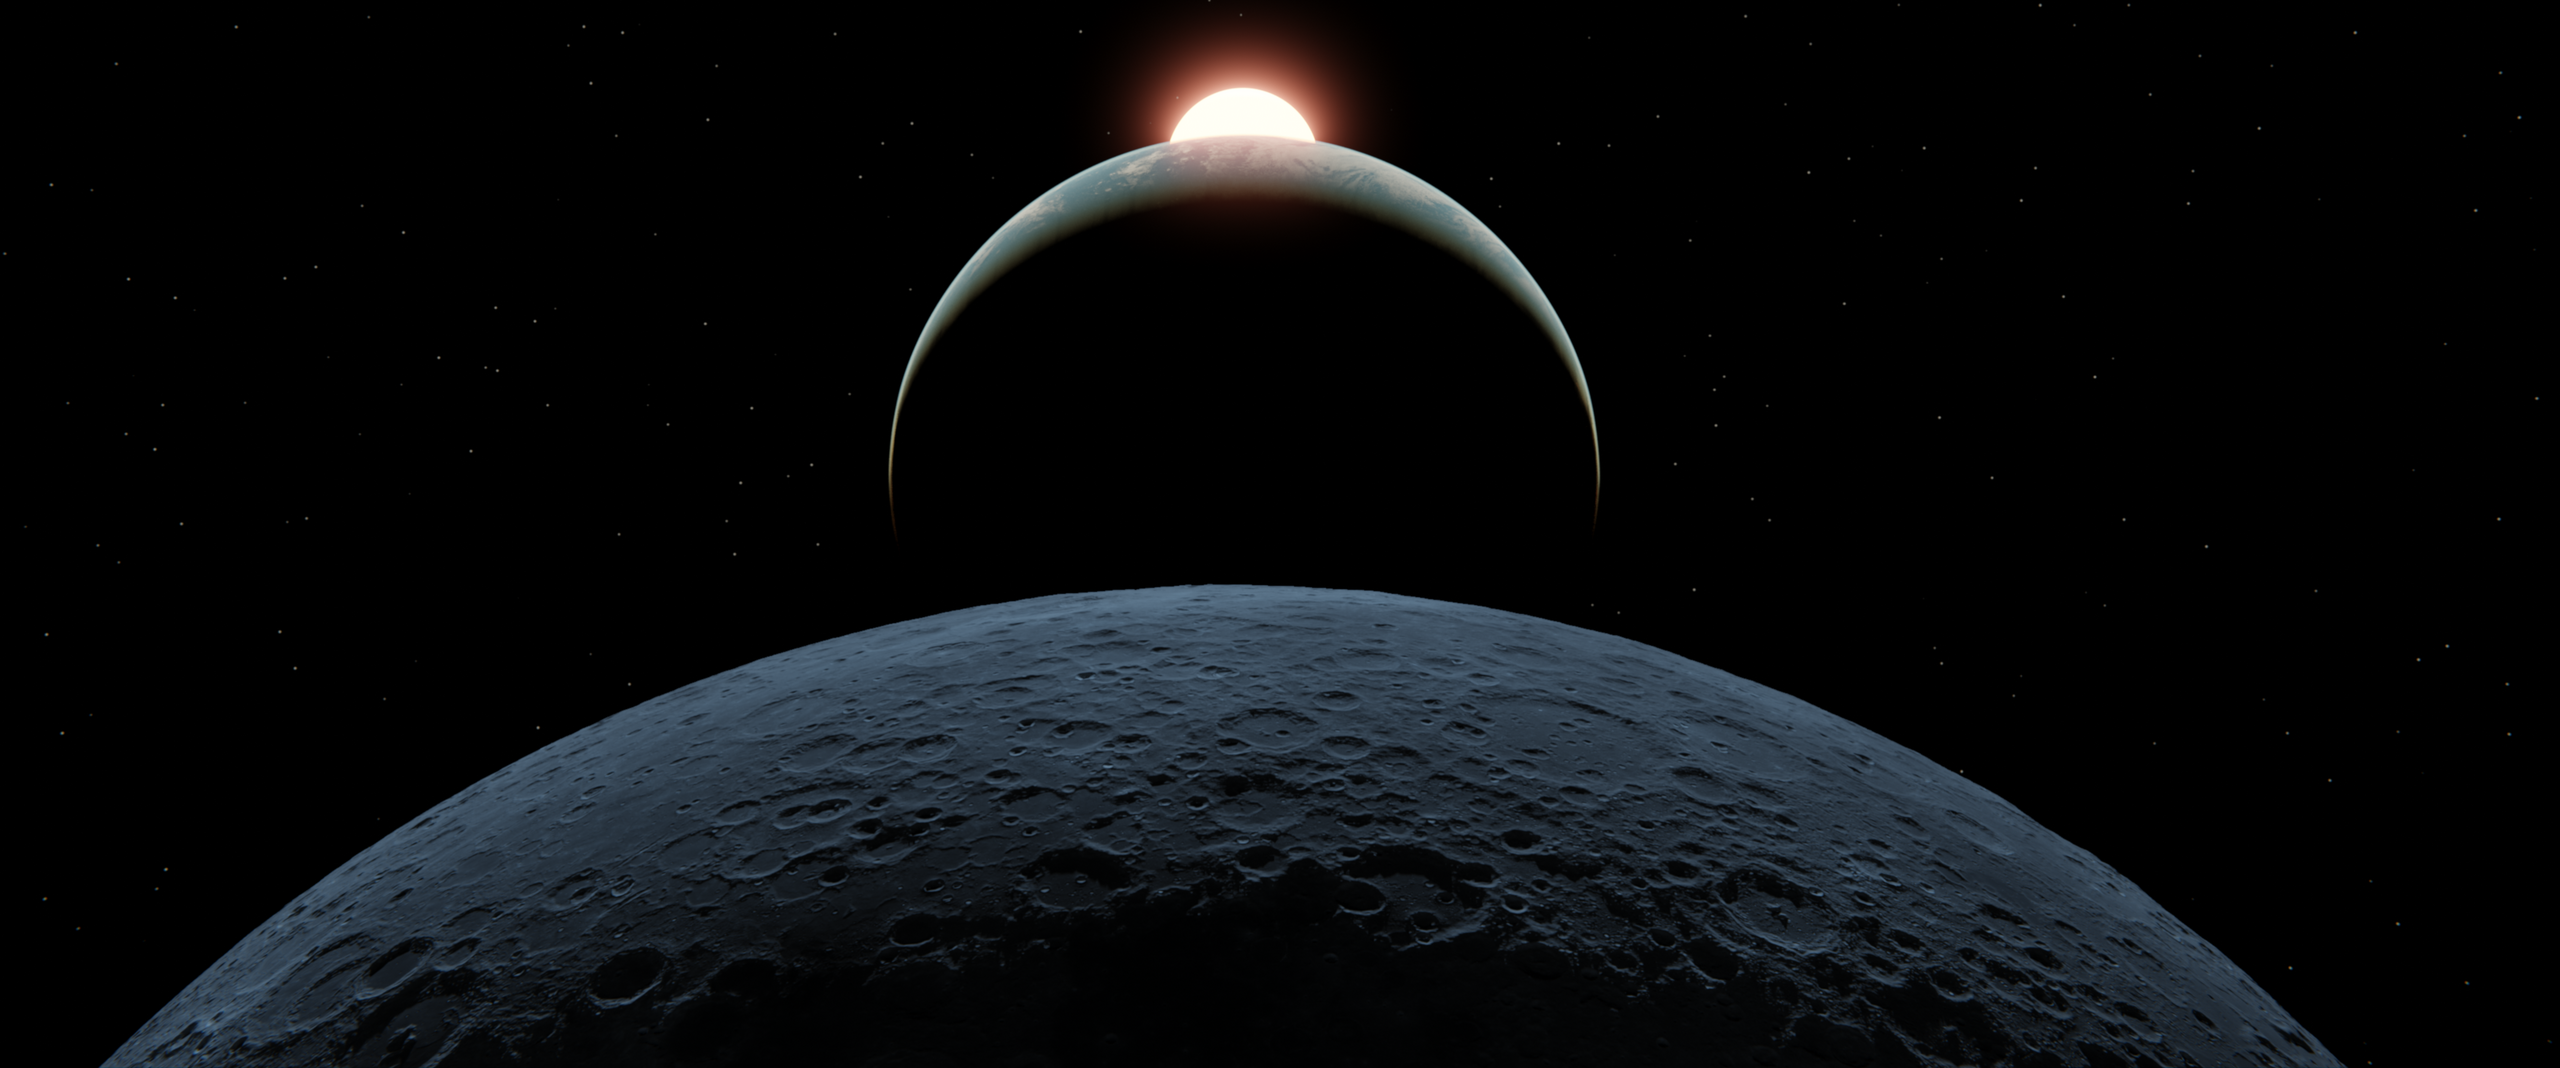
\includegraphics[width=1.25\textwidth]{./additional_graphics/Opening_2001-_A_Space_Odyssey.png}
		\creditdarknofill{A remake of the opening scene by SumoSebi, \href{https://commons.wikimedia.org/wiki/File:Opening_2001-_A_Space_Odyssey.png}{CC-BY-SA on Wikimedia Commons}}
	\end{figure}
	{\small	Stanley Kubrick's \emph{2001- A Space Odyssey} premieres  2 April 1968}

\end{frame}

\begin{frame}{1968: Nobel prize for the interpretation of the genetic code}
	\begin{columns}[T,onlytextwidth]
		\column{0.6\textwidth}
		\begin{figure}
			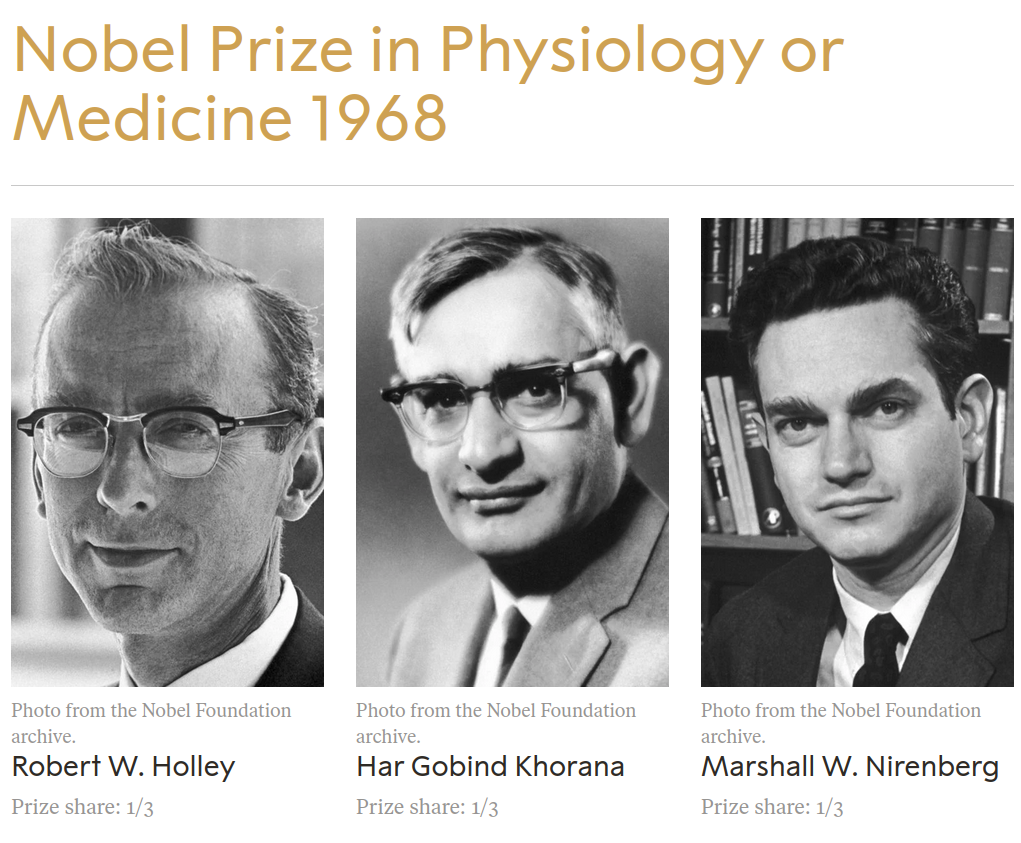
\includegraphics[width=\textwidth]{./figures/nobel1968.png}
		\end{figure}
		\column{0.5\textwidth}
		\begin{figure}
			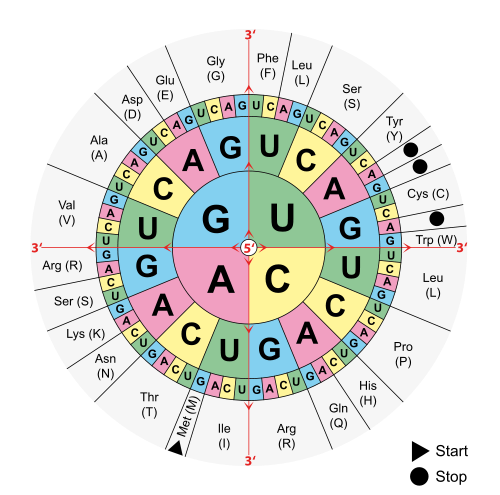
\includegraphics[width=\textwidth]{./figures/codesonne2.png}
		\end{figure}
	\end{columns}
	\begin{itemize}
		\item The genetic code is (almost) universal$^{[1]}$ 
		\item It was resolved entirely using synthetic sequences.
	\end{itemize}
	 \par {\scriptsize [1] \url{http://www.ncbi.nlm.nih.gov/Taxonomy/taxonomyhome.html/index.cgi?chapter=tgencodes}}
	\credit{\url{https://www.nobelprize.org/prizes/medicine/1968/summary} | User:Mouagip, Wikimedia Commons, PD}
\end{frame}

\begin{frame}{Encoded information of naturally occuring DNA unknown}
	\begin{columns}[T,onlytextwidth]
		\column{0.3\textwidth}
		\begin{figure}
			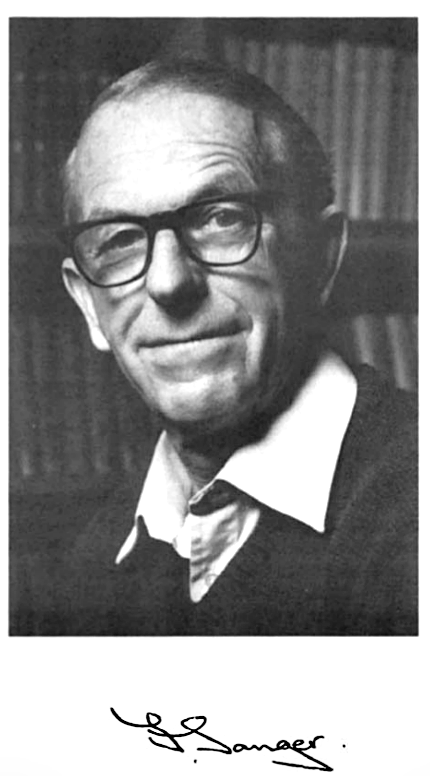
\includegraphics[width=\textwidth]{./figures/sanger.png}
		\end{figure}
		\column{0.7\textwidth}
		\vspace{3em}
		\begin{itemize}
			\item Peptides could be sequenced since the 
			1950s (Sanger method, Edman degradation).
			\item Sequencing of DNA was one of the most urgent, unresolved problems in the early 1970s.
			\item Frederick Sanger (Nobel laureate for sequencing Insulin 1958) started working with DNA. 
		\end{itemize}
	\end{columns}
\end{frame}

\begin{frame}{1977: Chain-termination sequencing by Frederick Sanger}
	\begin{columns}[T,onlytextwidth]
		\column{0.35\textwidth}
		\begin{figure}
			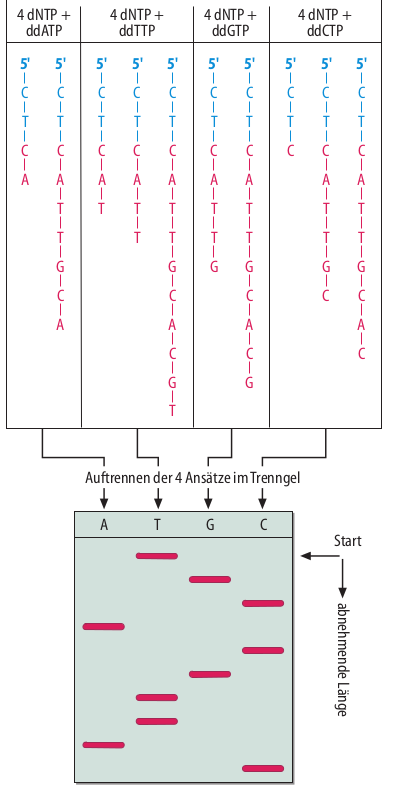
\includegraphics[width=\textwidth]{./figures/sangersequencing.png}
		\end{figure}
		\column{0.65\textwidth}
		\begin{itemize}
			\item DNA fragments could be separated by size.
			\item Sanger's method creates sequence-derived length patterns.
			\item It relies on radioactive labeling and in-vitro amplification of DNA.
		\end{itemize}
		\begin{figure}
			
\includegraphics[width=\textwidth]{./figures/sangerpaper.png}
			\caption{\citeme{Sanger1977}}
		\end{figure}
	\end{columns}
	\credit{$\leftarrow$ Fig.5.40, Löffler: Biochemie und Pathobiochemie 7th Ed.}
\end{frame}

\begin{frame}{1980: Nobel prize for DNA sequencing}
	\begin{columns}[T,onlytextwidth]
		\column{0.6\textwidth}
		\begin{figure}
			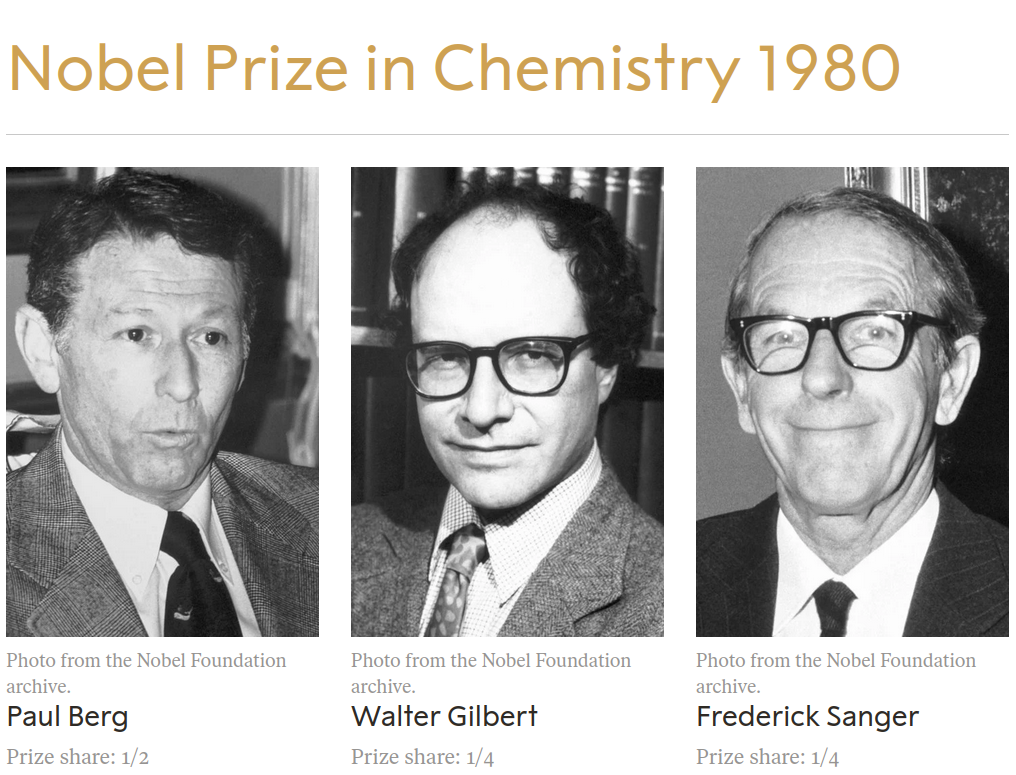
\includegraphics[width=\textwidth]{./figures/nobel-sanger.png}
		\end{figure}
		\column{0.5\textwidth}
		\begin{itemize}
			\item Ample DNA input needed\par {\scriptsize PCR was introduced in 1989}
			\item Four reactions per sequence
			\item Read length $\sim$ 200bp
		\end{itemize}
		\vspace{0.2cm}
		\begin{figure}
			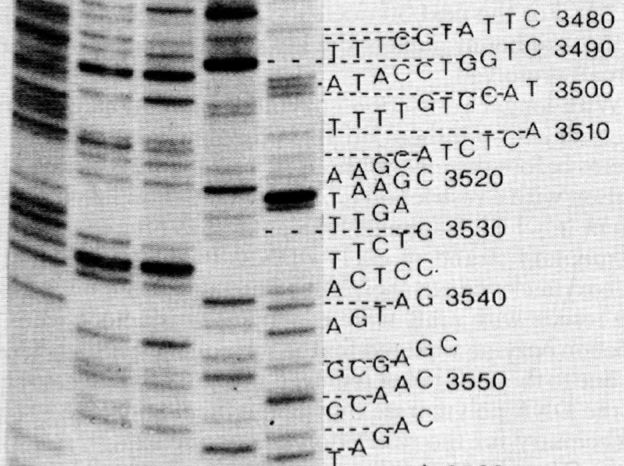
\includegraphics[width=0.8\textwidth]{./figures/sangergel.png}
		\end{figure}
	\end{columns}
 \creditleft{\url{https://www.nobelprize.org/prizes/chemistry/1980/summary}}
\end{frame}

\begin{frame}{Advanced Sanger sequencing for the Human Genome Project}
	\begin{columns}[T,onlytextwidth]
		\column{0.5\textwidth}
		\begin{figure}
			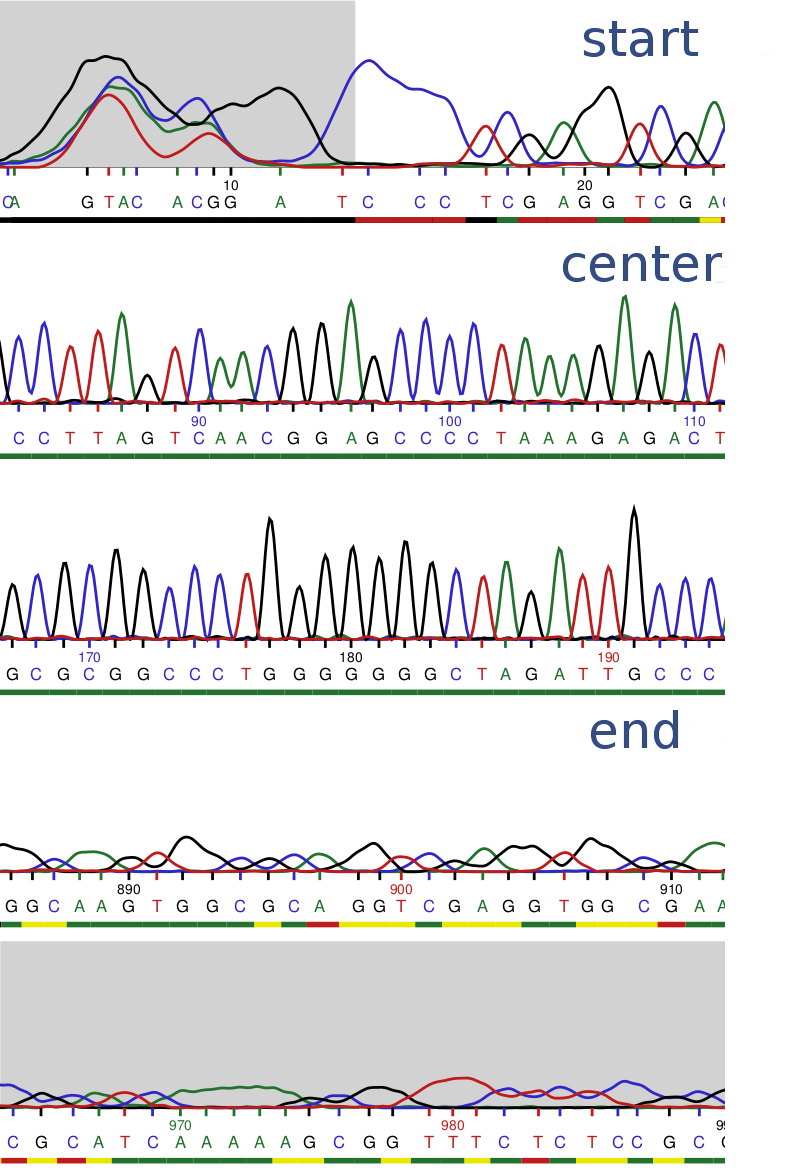
\includegraphics[width=\textwidth]{./figures/chromatogramm-eng.png}
		\end{figure}
		\column{0.5\textwidth}
		\begin{figure}
			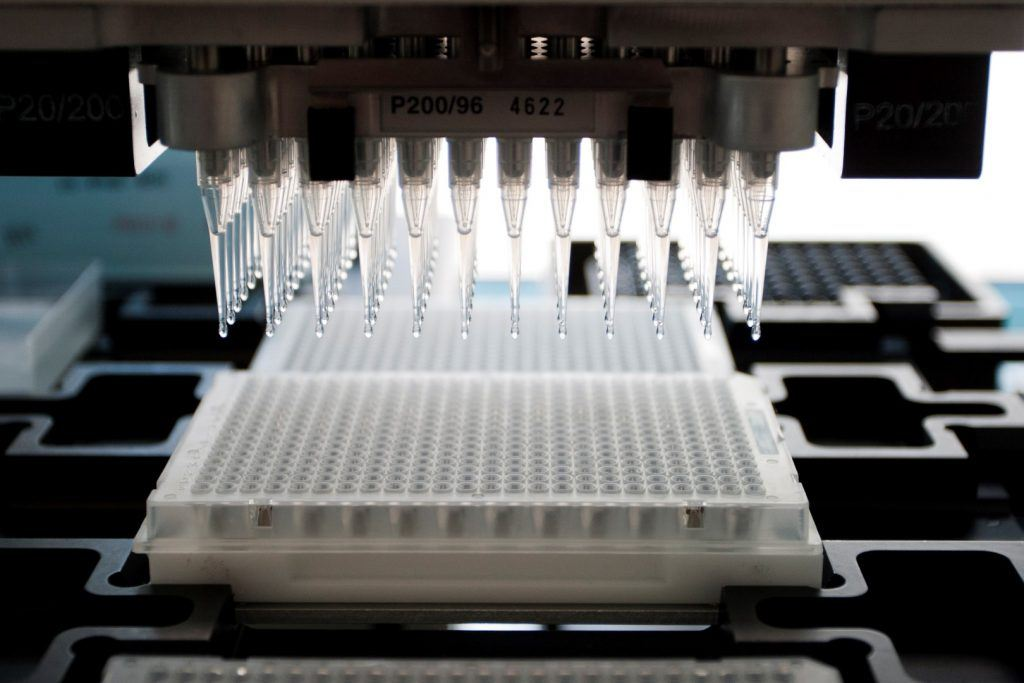
\includegraphics[width=\textwidth]{./figures/baseclearseq.jpg}
		\end{figure}
		\vspace{0.2cm}
		\begin{itemize}
			\item Fluorescent chain terminators.
			\item Capillary electrophoresis for size separation of amplicons.
			\item Parallelized and automated.
			\item Sequencing technology of the Human Genome Project (1990-2004).
		\end{itemize}
		\par \vspace{0.5cm}
		\credit{$\leftarrow$ A chromatogram generated by Sanger sequencing}
	\end{columns}
\end{frame}

% % % % % % % % % % % % % % % % % % % % % %  % % % % % % % % % %

\section{Next-generation sequencing}

% % % % % % % % % % % % % % % % % % % % % % % % % % % % % % % % % 

\begin{frame}{New high-throughput methods were developed}
	\begin{center}
		 \begin{figure}
		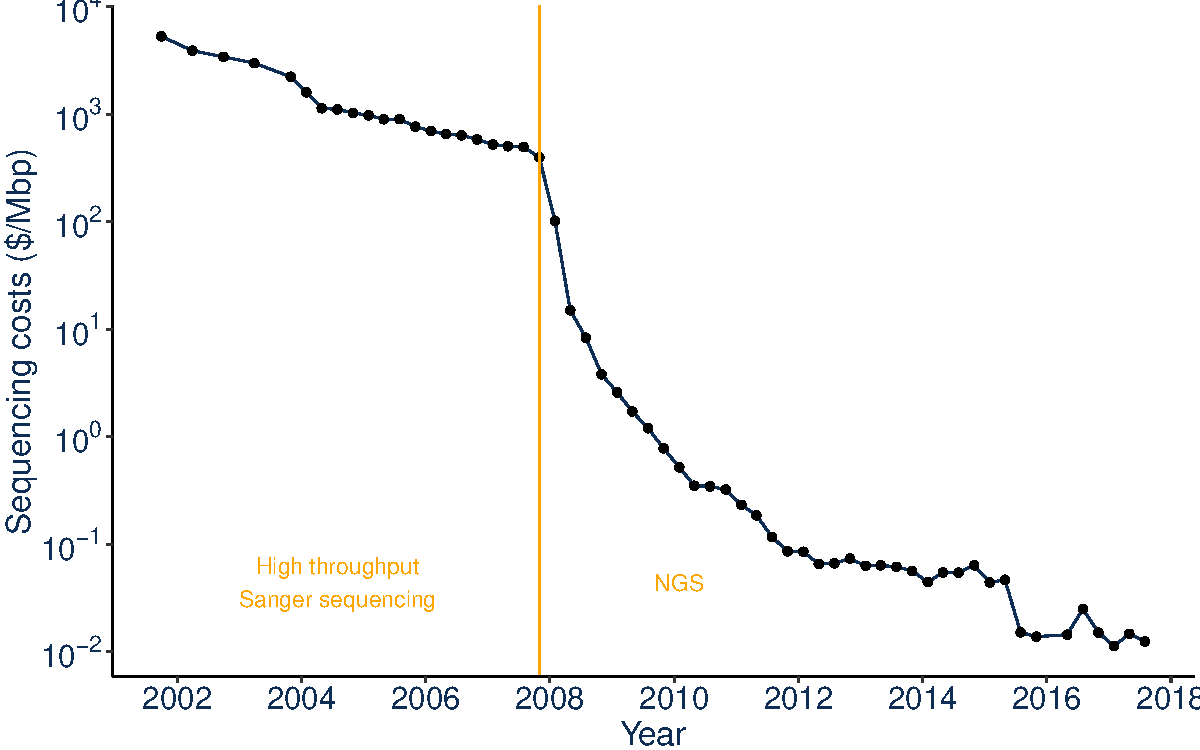
\includegraphics[width=0.7\textwidth]{./figures/sequencingcosts2018eng.pdf}
		\caption{Sequencing costs per one million bases of raw sequence}
		\end{figure}
	\end{center}
    \begin{description}
	\item [1990-2004:] Human Genome Project sequencing: US \$500 million
	\item [2025:] Sequencing of a human genome: $\sim$ US \$100-1000
\end{description}
	\credit{National Human Genome Research Institute (NHGRI) \linebreak \href{https://www.genome.gov/about-genomics/fact-sheets/Sequencing-Human-Genome-cost}{https://www.genome.gov/about-genomics/fact-sheets/Sequencing-Human-Genome-cost}}
\end{frame}

\begin{frame}{Around 2010: Sanger sequencing was outcompeted by NGS}
	\begin{columns}[T,onlytextwidth]
		\column{0.5\textwidth}
		\begin{figure}
			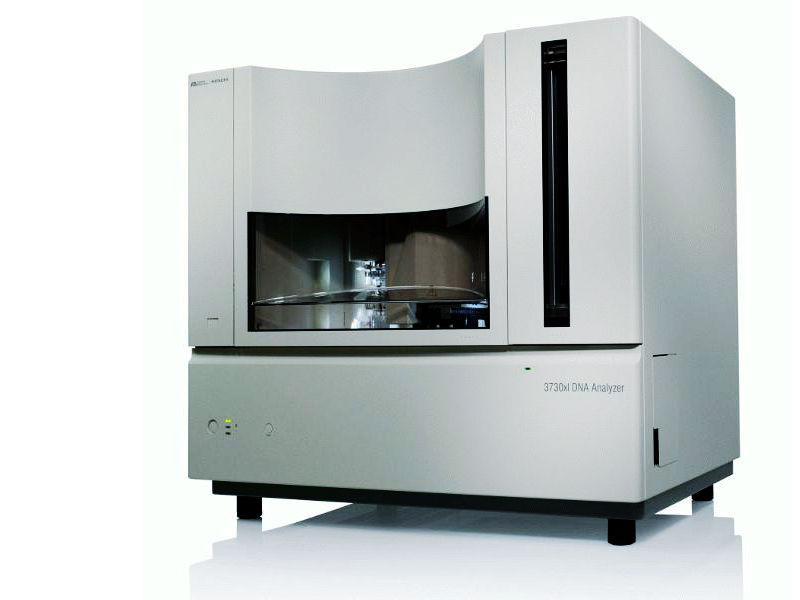
\includegraphics[width=0.8\textwidth]{./figures/abi3730xl.jpg} \vspace{1em} \\
		\end{figure}
		\column{0.5\textwidth}
		\begin{figure}
			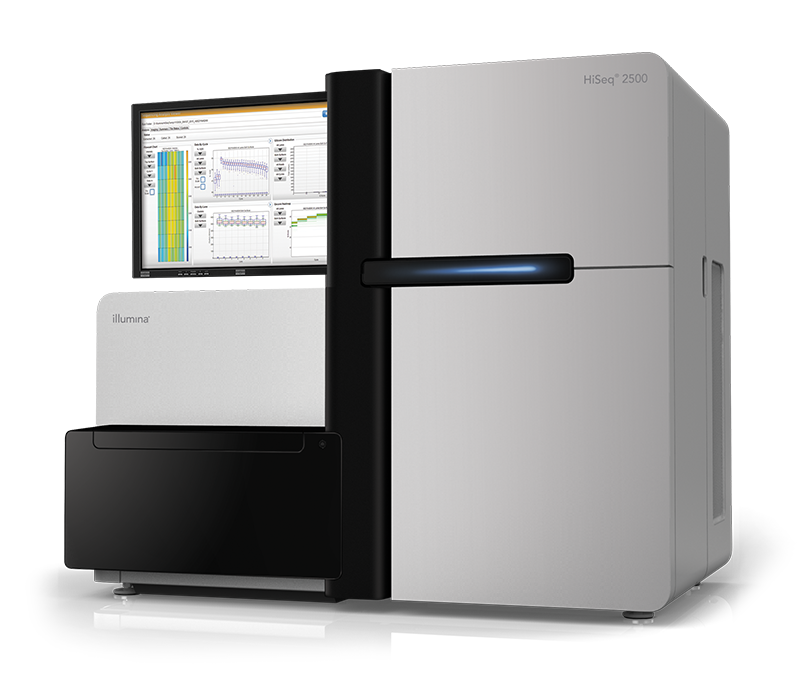
\includegraphics[width=0.8\textwidth]{./figures/system-carousel-hiseq2500-left.png}
		\end{figure}
	\end{columns}
	\begin{columns}[T,onlytextwidth]
		\column{0.5\textwidth}
		\begin{exampleblock}{}
			\textbf{ABI 3730xl DNA Sequencer}\\
			(Sanger Multiplex, 2013)
			\begin{itemize}
				\item $\sim$6912 reads of 400bp
				\item $\sim$2,76 Mbp / day
			\end{itemize}
		\end{exampleblock}
		\column{0.5\textwidth}
		\begin{exampleblock}{}
			\textbf{Illumina HiSeq 2500}  \vspace{0.3em} \\
			(NGS / MPS, 2013)
			\begin{itemize}
				\item $\sim$600 Million reads of 100bp
				\item $\sim$60.000 Mbp / day
			\end{itemize}
			{ \small (depending on settings and sequencing chemistry used)}
		\end{exampleblock}
	\end{columns}
\end{frame}

% % % % % % % % % % % % % % % % % % % % % % % 

\section{National Genomics Infrastructure Sweden}

% % % % % % % % % % % % % % % % % % % % % % % 

\begin{frame}{DNA sequencing facilities provide sequencing capacity}
	\begin{center}
	\hspace*{-1cm}
	
\includegraphics[height=0.2\textheight]{./additional_graphics/NGI-logo.png}
	\end{center}
	\begin{itemize}
		\item DNA sequencing of paramount importance for life science.
		\item 2013: National Genomics Infrastructure Sweden is founded.
		\item Our mission is to offer a state-of-the-art infrastructure available to researchers all over Sweden.
     \end{itemize}
\end{frame}

\begin{frame}{Users of the National Genomics Infrastructure Sweden}
	\begin{center}
		\hspace*{-1cm}
		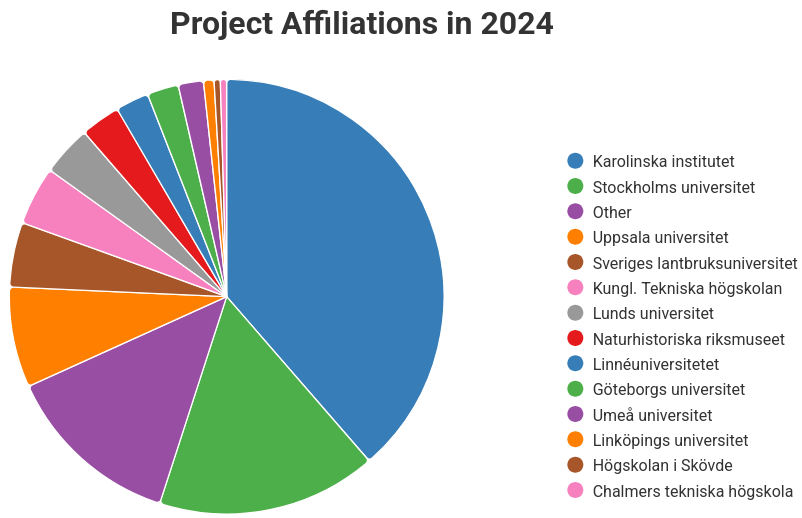
\includegraphics[height=0.7\textheight]{./figures/ngi-users-2024.png}
	\end{center}
	\credit{\href{https://ngisweden.scilifelab.se/resources/ngi-stockholm-status/}{https://ngisweden.scilifelab.se/resources/ngi-stockholm-status/}}
\end{frame}

\begin{frame}{National Genomics Infrastructure Sweden}
  \begin{columns}[T]
     \column{0.6\textwidth}
	\begin{center}
		\hspace*{-1cm}
		
\includegraphics[height=0.2\textheight]{./additional_graphics/NGI-logo.png}
	\end{center}
	\begin{itemize}
		\item NGI is a sequencing facility for \emph{research projects} 
		\item Part of the Genomics Platform at SciLifeLab
		\item Distributed in 3 nodes:
		\begin{itemize}
			\item SNP\&SEQ Technology Platform, Uppsala
			\item Uppsala Genome Center
			\item NGI Stockholm + Eukaryotic Single Cell Genomics (ESCG), Solna 
		\end{itemize}
	\end{itemize}
       \column{0.5\textwidth}
       \vspace*{2cm}
       
\includegraphics[width=\textwidth]{./figures/scilifelab-map.png} 
    \end{columns}
	\credit{\href{https://ngisweden.scilifelab.se}{https://ngisweden.scilifelab.se}}
\end{frame}

\begin{frame}{NGI-S employs various sequencing technologies}
	\begin{center}
		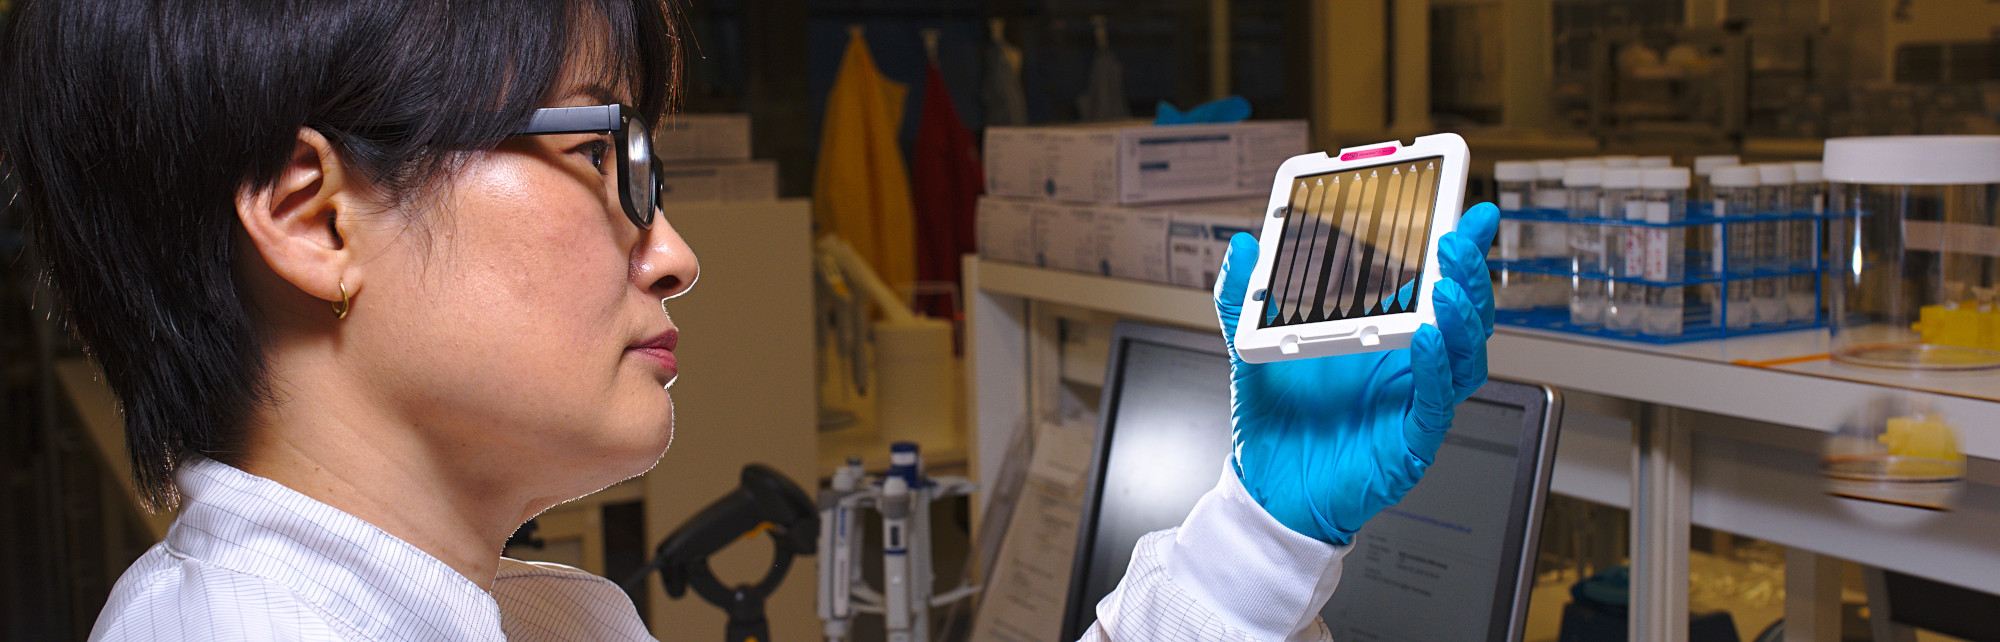
\includegraphics[width=0.7\textwidth]{./figures/ngi-choi-flowcell.jpg} \\
		\hspace*{-1cm}
		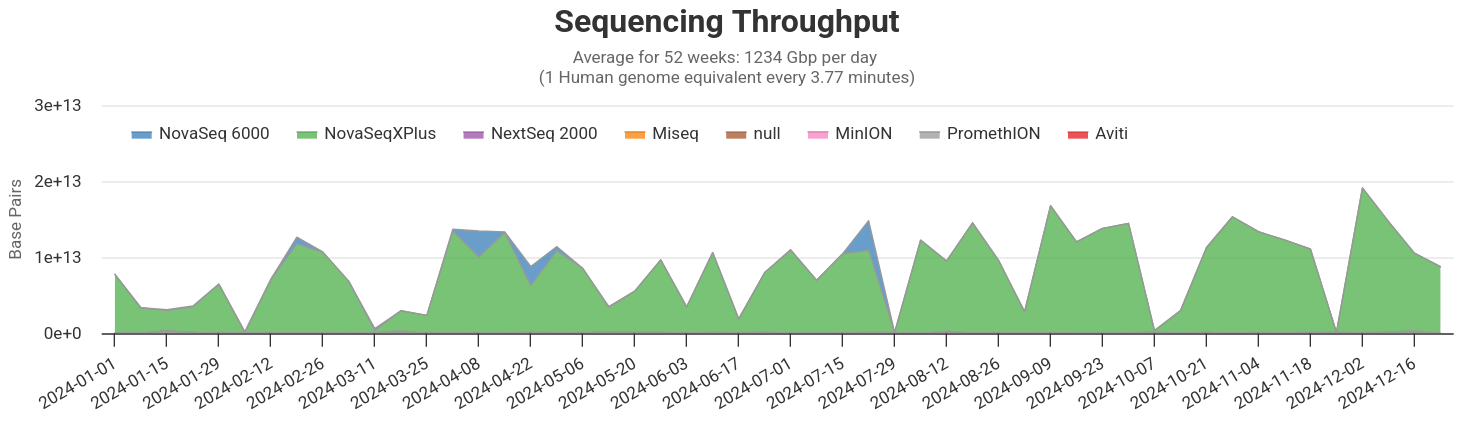
\includegraphics[width=1.2\textwidth]{./figures/ngis-throughput-2024.png}
	\end{center}
	\begin{itemize}
		\item In 2024, NGI Stockholm sequenced on average 1200 Gbp/day
	\end{itemize}
	\credit{\href{https://ngisweden.scilifelab.se/resources/ngi-stockholm-status/}{https://ngisweden.scilifelab.se/resources/ngi-stockholm-status/}}
\end{frame}

% % % % % % % % % % % % % % % % % % % % % % % 

\section{Sequencing platforms}

% % % % % % % % % % % % % % % % % % % % % % % 

\begin{frame}{Sequencing platforms / technologies since Sanger}
	%\metroset{block=fill}
	\begin{exampleblock}{Next generation sequencing}
		\begin{itemize}
			\item Roche 454 sequencing (Pyrosequencing)
			\item Ion semiconductor sequencing
			\item \textbf{Illumina (Solexa) sequencing}
			\item \textbf{PacBio HiFi Sequencing}
		\end{itemize}
	\end{exampleblock}
	\begin{alertblock}{Third generation sequencing}
		\begin{itemize}
			\item \textbf{Oxford Nanopore sequencing}
			\item \textbf{Element Biosciences Avidite Sequencing}
			\item Ultima Genomics UG 100 Sequencing
			\item MGI DNBSEQ Technology
			\item Singular Genomics G4X
		\end{itemize}
	\end{alertblock}
\credit{Platforms in \textbf{bold} are in use at the National Genomics Infrastructure}
\end{frame}

\begin{frame}{Sequencing platforms / technologies since Sanger}
	%\metroset{block=fill}
	\begin{exampleblock}{Sequencing by synthesis}
		\begin{itemize}
			\item Roche 454 sequencing (Pyrosequencing)
			\item Ion semiconductor sequencing
			\item \textbf{Illumina (Solexa) sequencing}
			\item \textbf{PacBio HiFi Sequencing}
			\item \textbf{Element Biosciences Avidite Sequencing}
			\item Ultima Genomics UG 100 Sequencing
			\item MGI DNBSEQ Technology
			\item Singular Genomics G4X
		\end{itemize}
	\end{exampleblock}
	\begin{alertblock}{Direct DNA/RNA sequencing}
		\begin{itemize}
			\item \textbf{Oxford Nanopore sequencing}
		\end{itemize}
	\end{alertblock}
\credit{Platforms in \textbf{bold} are in use at the National Genomics Infrastructure}
\end{frame}

\begin{frame}{Illumina sequencing is \emph{the} NGS sequencing platform}
	\begin{center}
		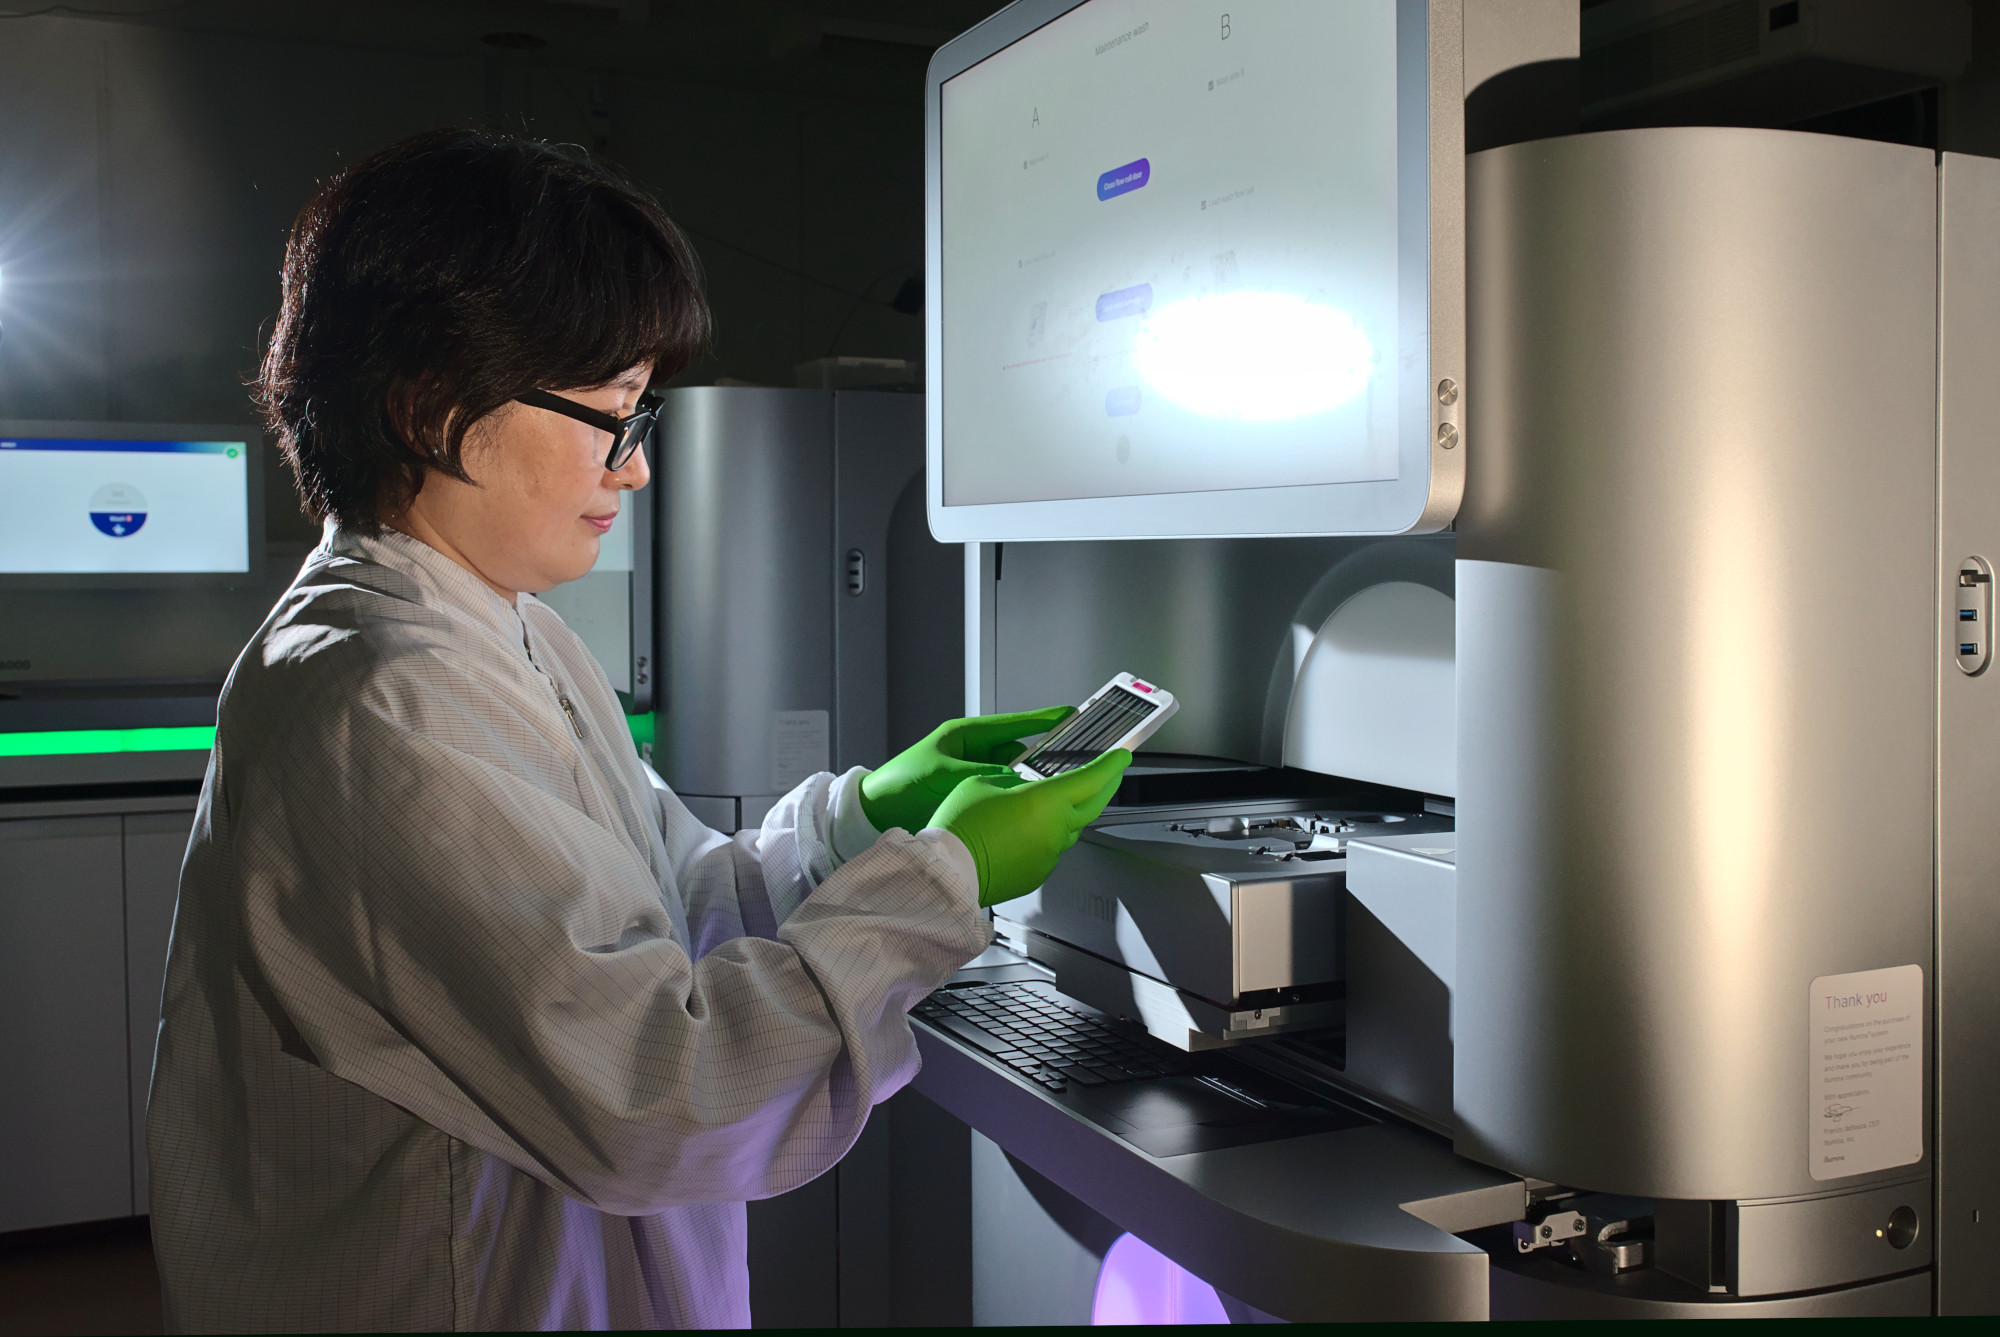
\includegraphics[width=0.7\textwidth]{./figures/ngi-choi-novaseqxplus.jpg} \\
		\hspace*{-1cm}
		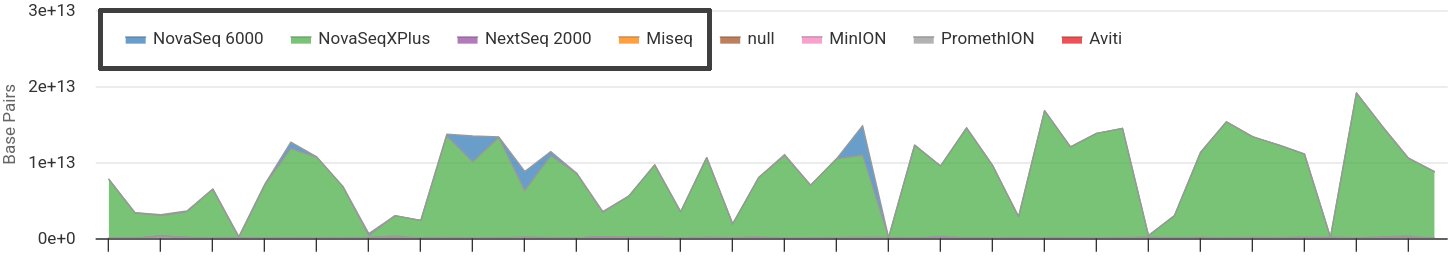
\includegraphics[width=1.2\textwidth]{./figures/ngis-throughput-2024-illumina.png}
	\end{center}
\creditleft{Illumina's sequencing by synthesis technology is NGI's bread-and-butter platform}
\end{frame}

\begin{frame}[standout]{Preparation for sequencing (in the lab)}
	\begin{columns}[T,onlytextwidth]
		\hspace*{-0.7cm} 
		\column{0.6\textwidth}
		\begin{figure}
			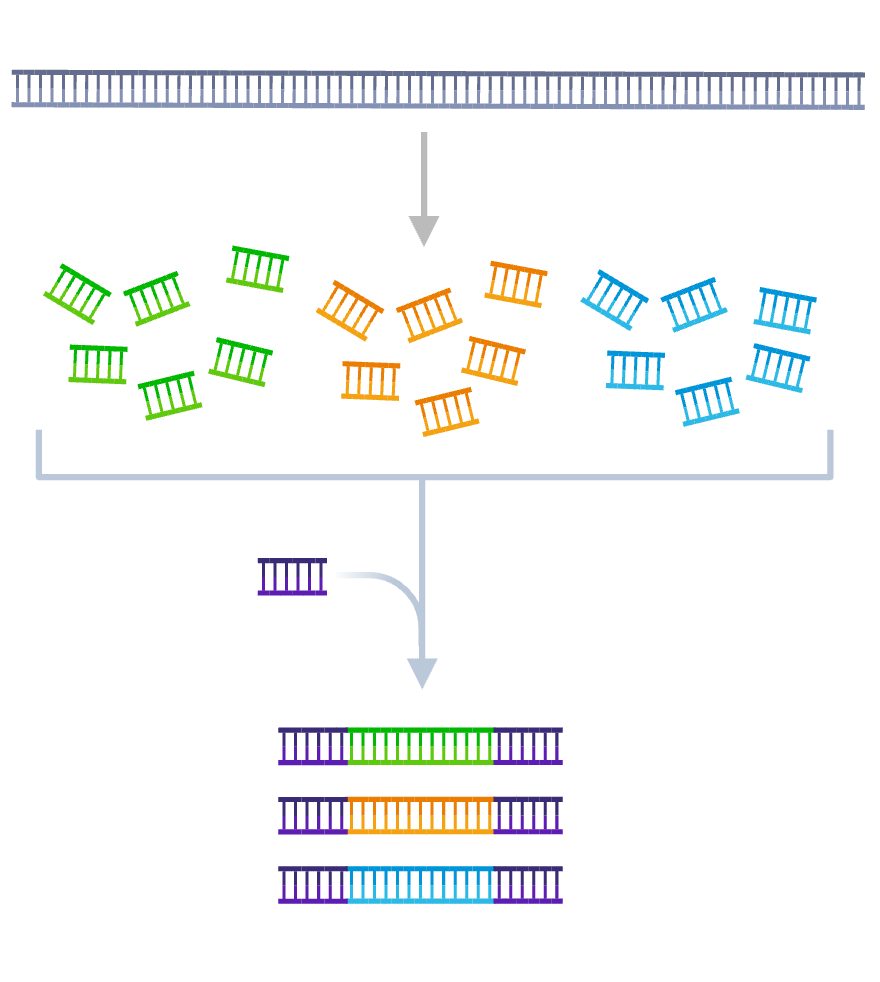
\includegraphics[width=\textwidth]{figures/library-prep.png}
		\end{figure}
		\column{0.5\textwidth}
			\normalsize \normalfont
			\begin{itemize}
				\item Experiment-specific isolation, purification and enrichment
				\item Fragmentation
				\begin{itemize}
					\item Enzymatic
					\item Mechanic
				\end{itemize}
				\item Addition of sequencing adapters 
				\begin{itemize}
					\item For attaching to the instrument
					\item Barcodes for sample multiplexing
					\item Unique Molecular Identifiers tag individual DNA fragments
				\end{itemize}
				\item Pooling of samples
			\end{itemize}
	\end{columns}
\creditdarkleft{Figure by Anja Mezger}
\end{frame}

\begin{frame}[standout]{Preparation for sequencing (on the machine)}
	\begin{columns}[T,onlytextwidth]
		\hspace*{-0.7cm} 
		\column{0.5\textwidth}
		\begin{figure}
			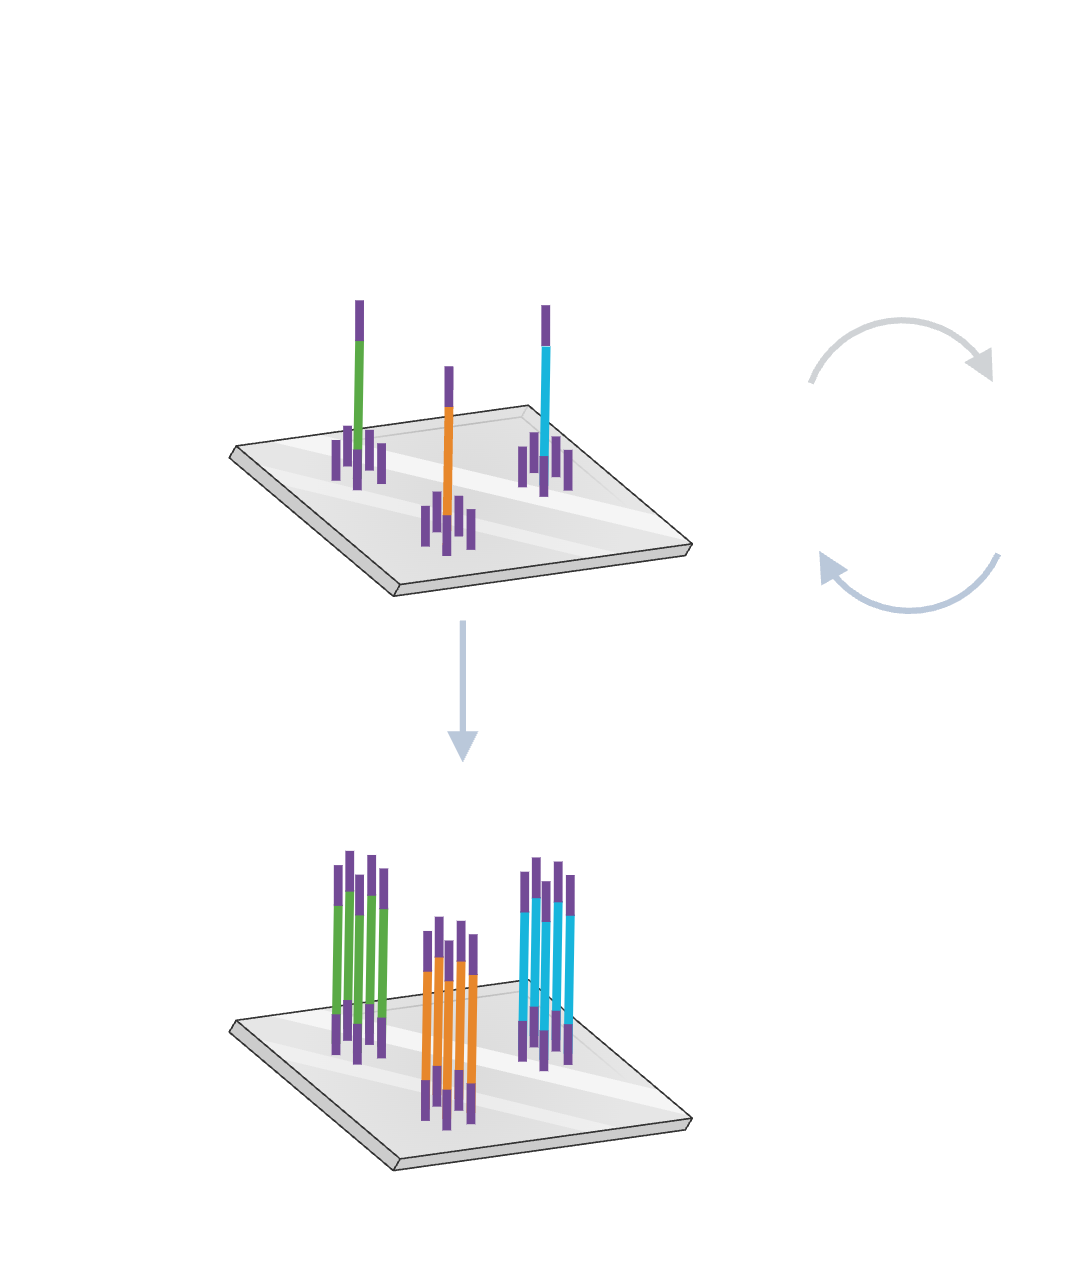
\includegraphics[width=\textwidth]{figures/bridge-amp.png}
		\end{figure}
		\column{0.52\textwidth}
		\normalsize \normalfont
		\begin{itemize}
			\item Hybridize to a \emph{flow cell} 
			\item Amplify for better signal
			\item Linearize
		\end{itemize}
		\vspace{1cm} \par
		\hspace{2em}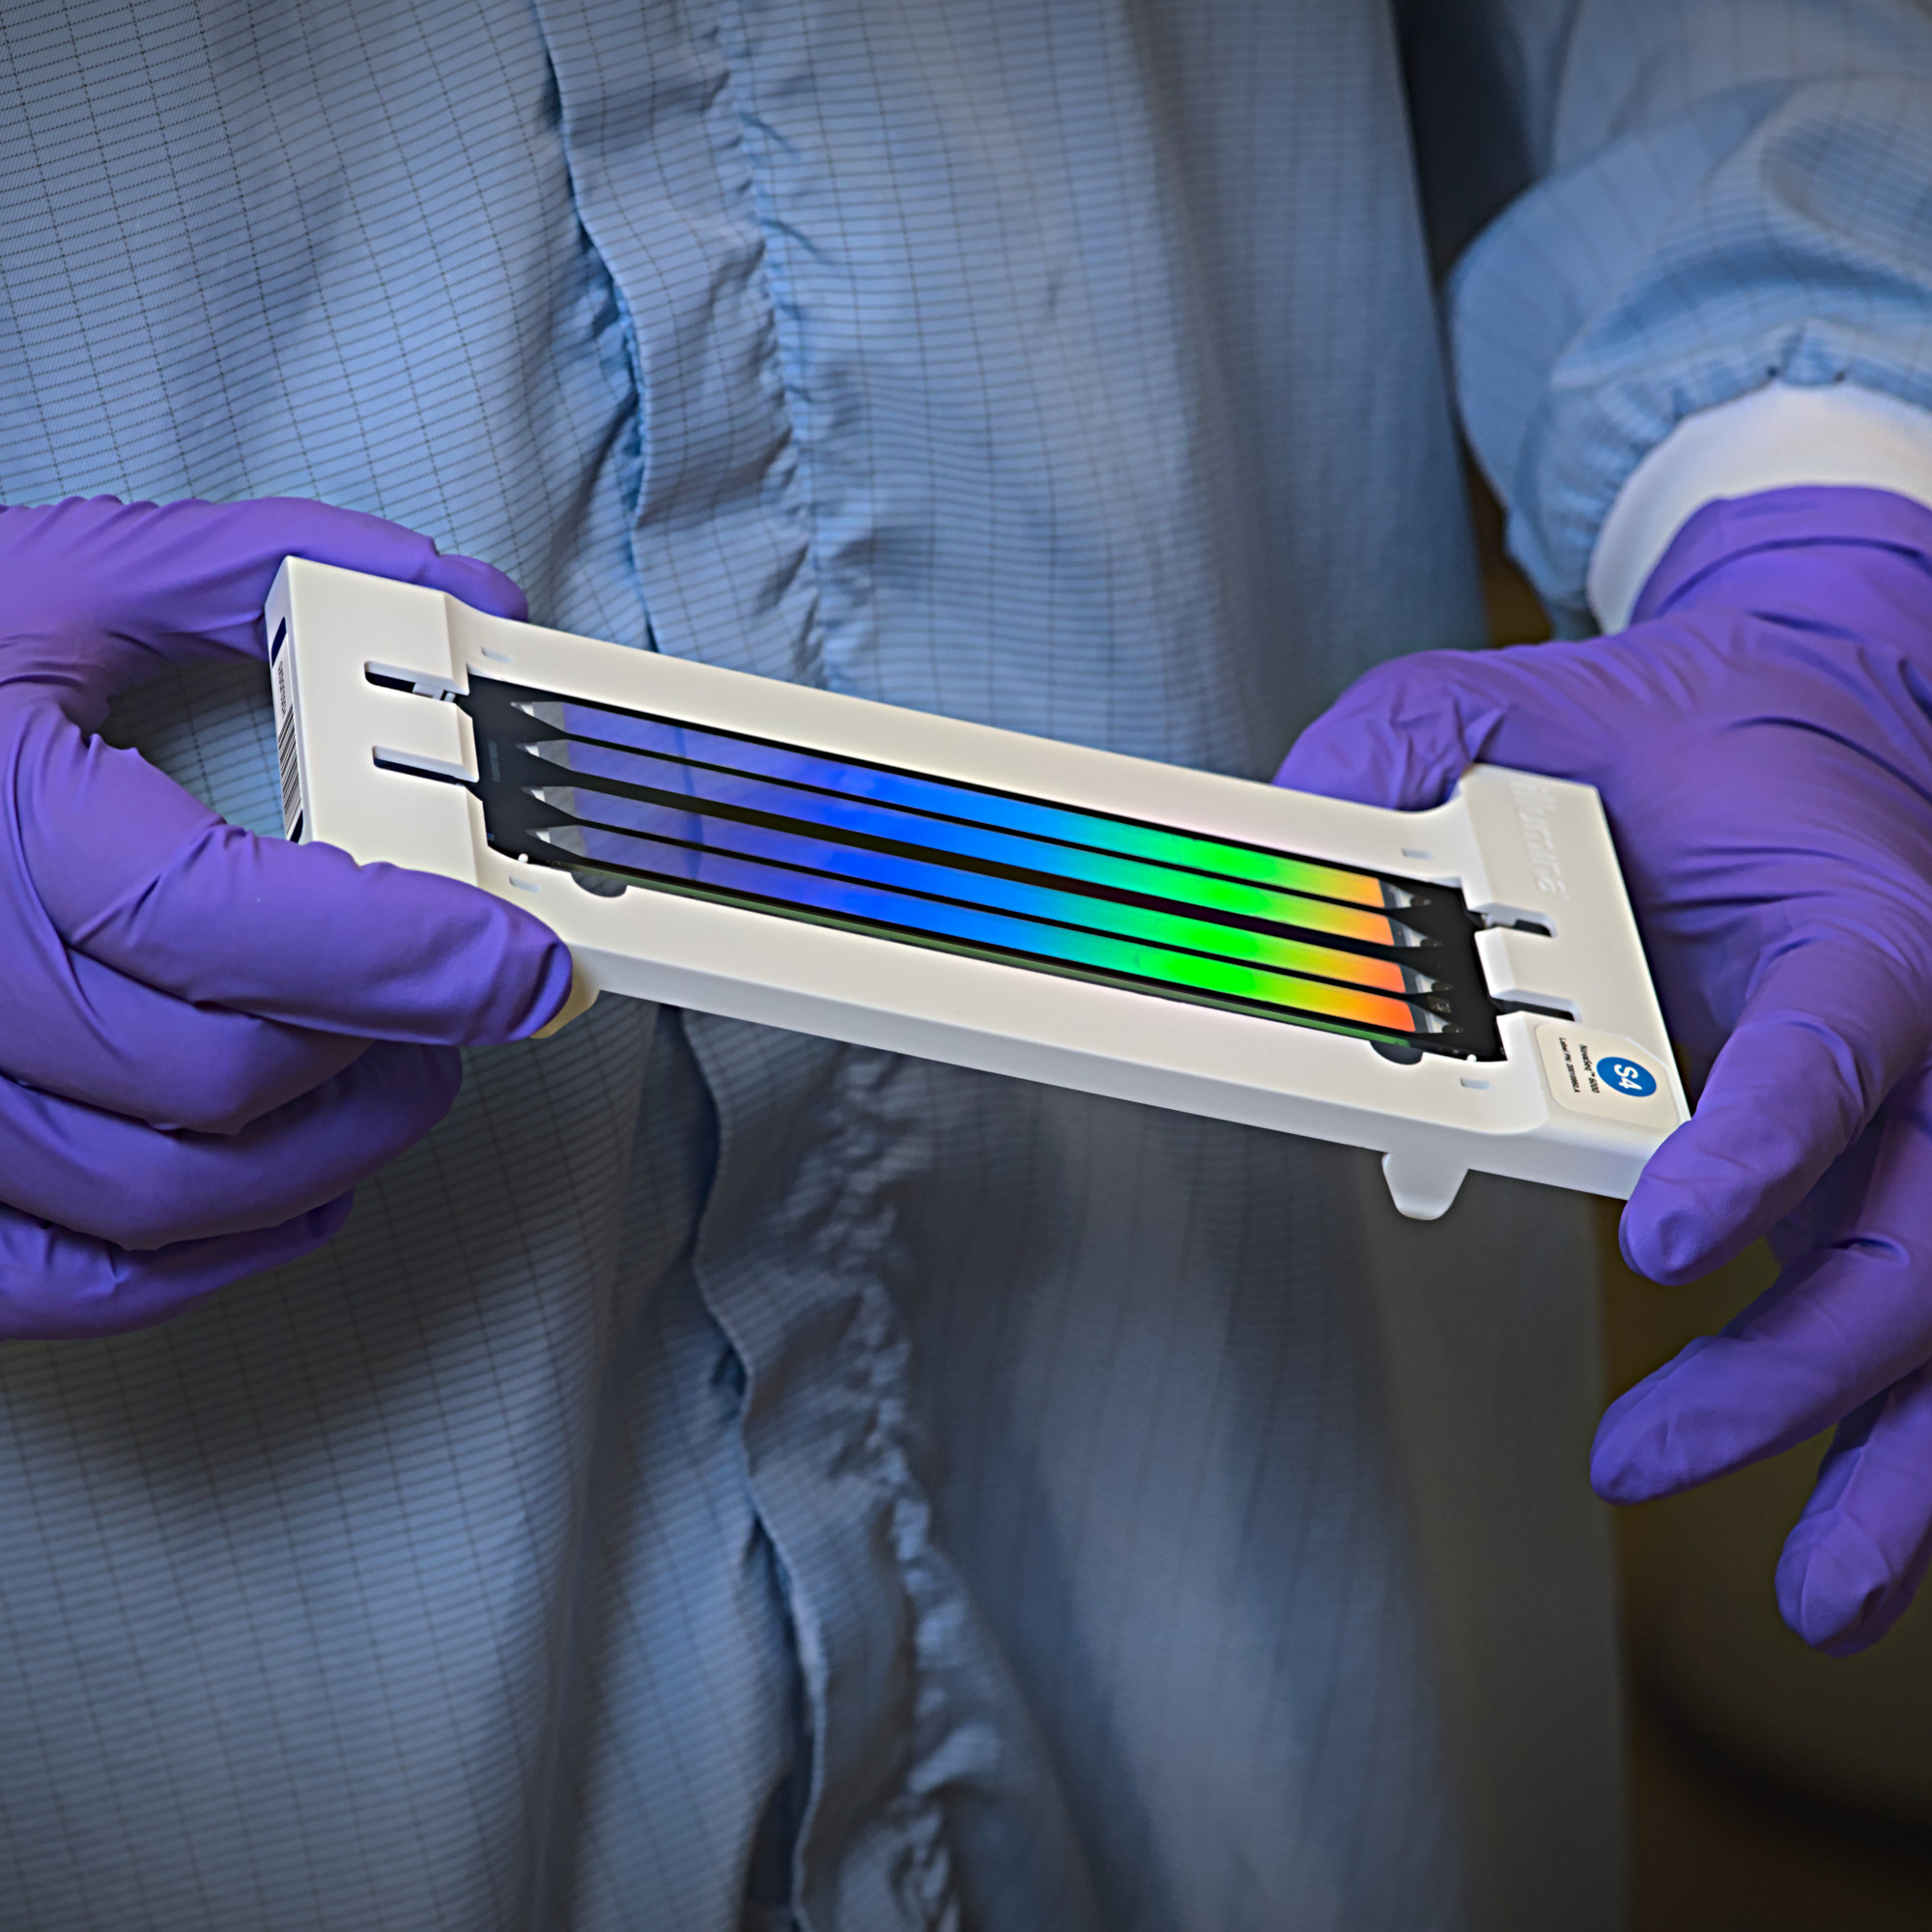
\includegraphics[width=0.7\textwidth]{./figures/flow_cell_3b.jpg}
	\end{columns}
\creditdarkleft{Figure by Anja Mezger}
\end{frame}

\begin{frame}[standout]{Illumina: \textit{Sequencing by Synthesis} of DNA clusters}
	\begin{columns}[T,onlytextwidth]
		\hspace*{-0.7cm} 
		\column{0.5\textwidth}
		\begin{figure}
			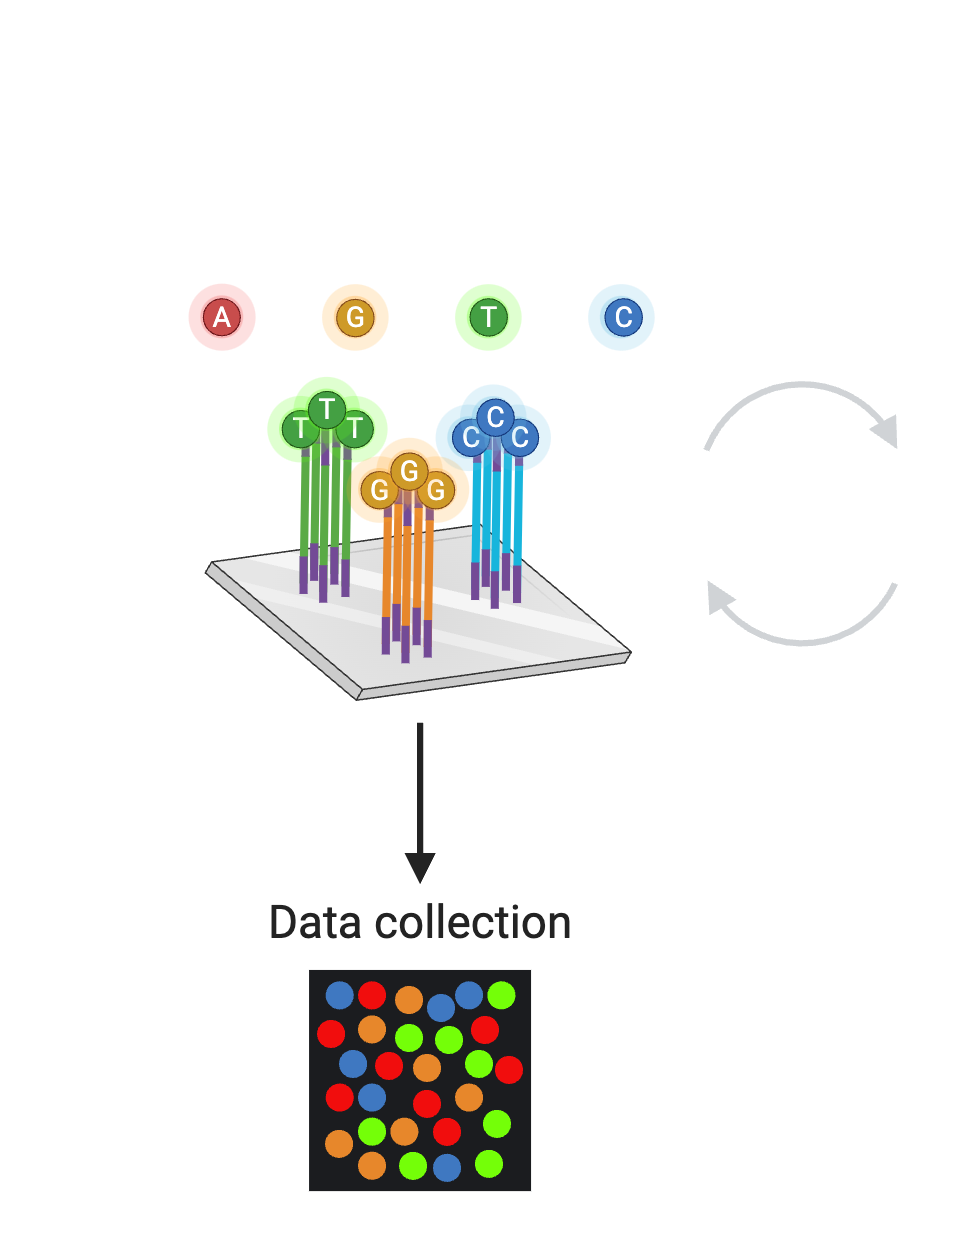
\includegraphics[width=\textwidth]{figures/ngs-cycles.png}
		\end{figure}
		\column{0.52\textwidth}
		\normalsize \normalfont
		\begin{itemize}
			\item DNA is amplified (again)
			\item Base integration yields a light signal (details vary among Illumina machines)
			\item Sequence is derived from a time-series of images
			\item NGS was developed from Sanger sequencing, but several key innovations were required.\citeme{Rodriguez2023}
		\end{itemize}
	\end{columns}
 	\creditdark{doi: 10.1038/s41587-023-01986-3} \par
	\creditdarkleft{Figure by Anja Mezger}
\end{frame}

\begin{frame}{Illumina: \textit{Sequencing by Synthesis} of DNA clusters}
	\begin{columns}[T]
		\column{\dimexpr\paperwidth-10pt}
		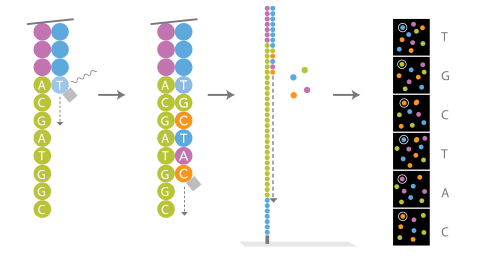
\includegraphics[width=0.6\textwidth]{./figures/illumina3.png}
		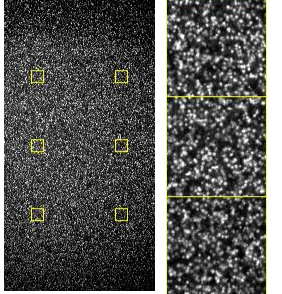
\includegraphics[width=0.37\textwidth]{./figures/flowcell.jpg}
	\end{columns}
	\begin{columns}[T,onlytextwidth]
		\column{\textwidth}
		\vspace{2em}
		\begin{enumerate}
			\item Integration of base is monitored directly
			\item Image sequence is recorded  
			\item For each cluster, the light/dark pattern is converted into a DNA sequence
		\end{enumerate}
		\alert{$\rightarrow$ Highly parallelized, direct monitoring as synthesis proceeds}
	\end{columns}
\end{frame}

\begin{frame}{\textit{Flow cells} instead of plates: Massive parallel sequencing}
	\begin{columns}[T]
		\column{\dimexpr\paperwidth-10pt}
	\begin{figure}
		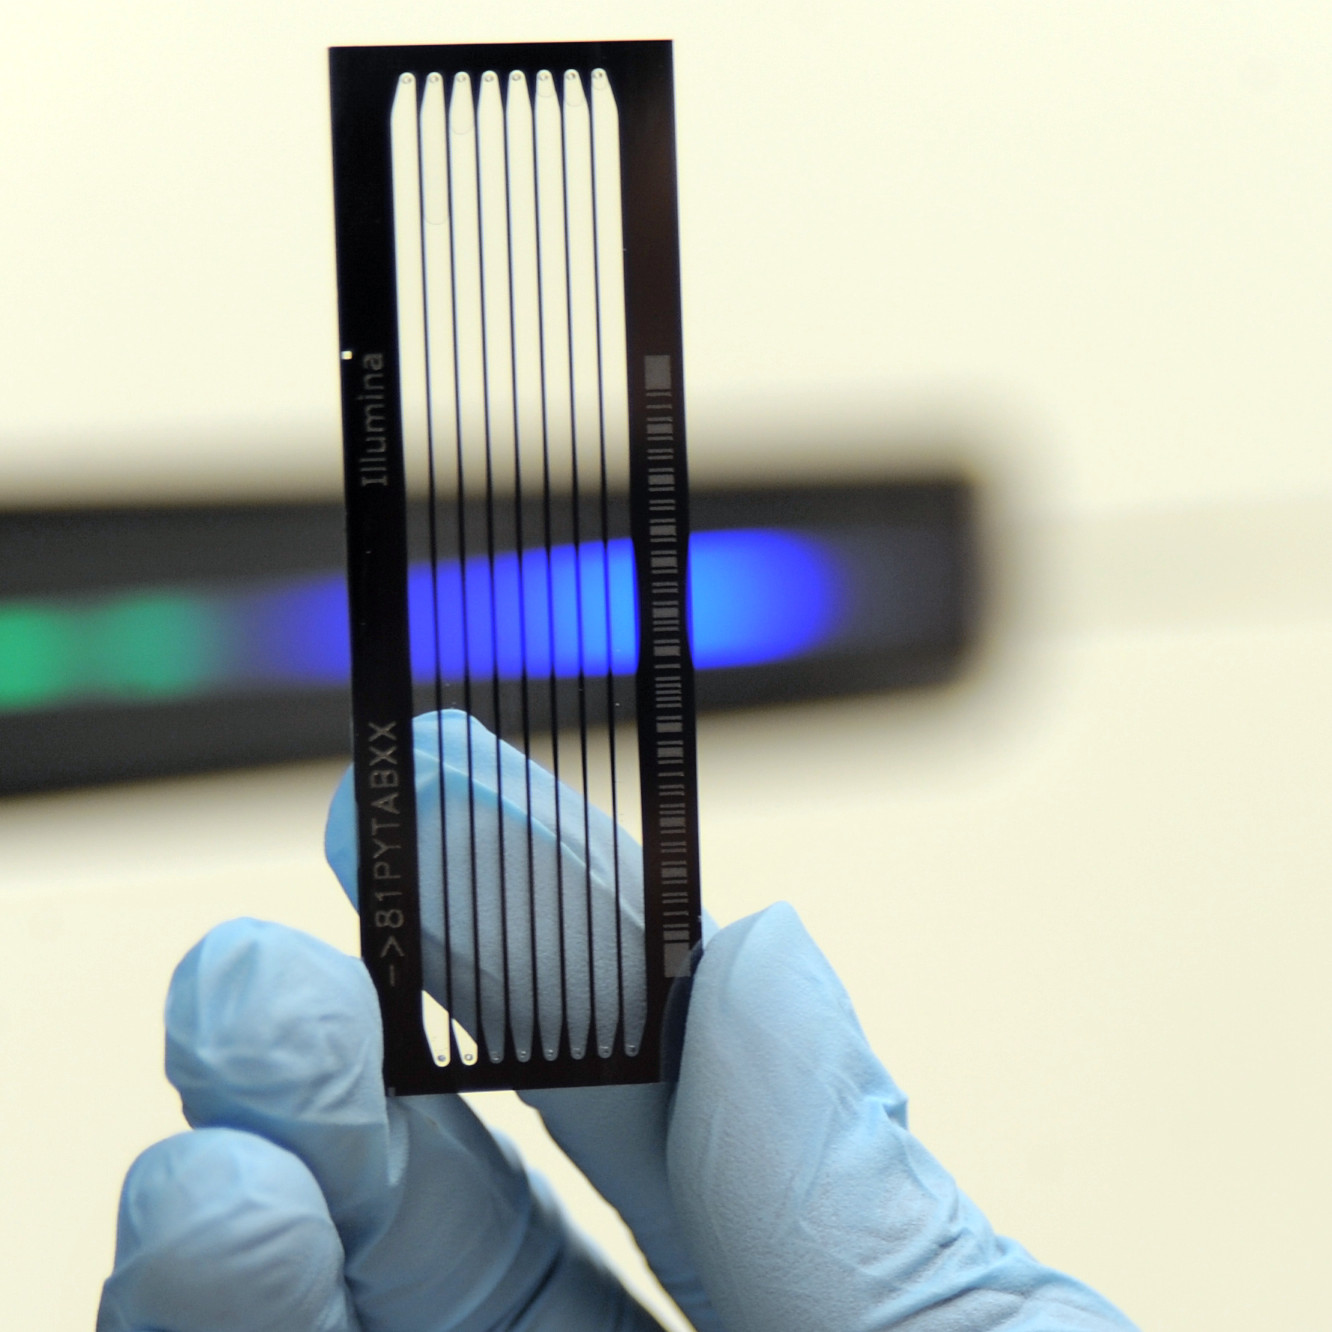
\includegraphics[width=0.24\textwidth]{./figures/flow_cell_1.jpg}
		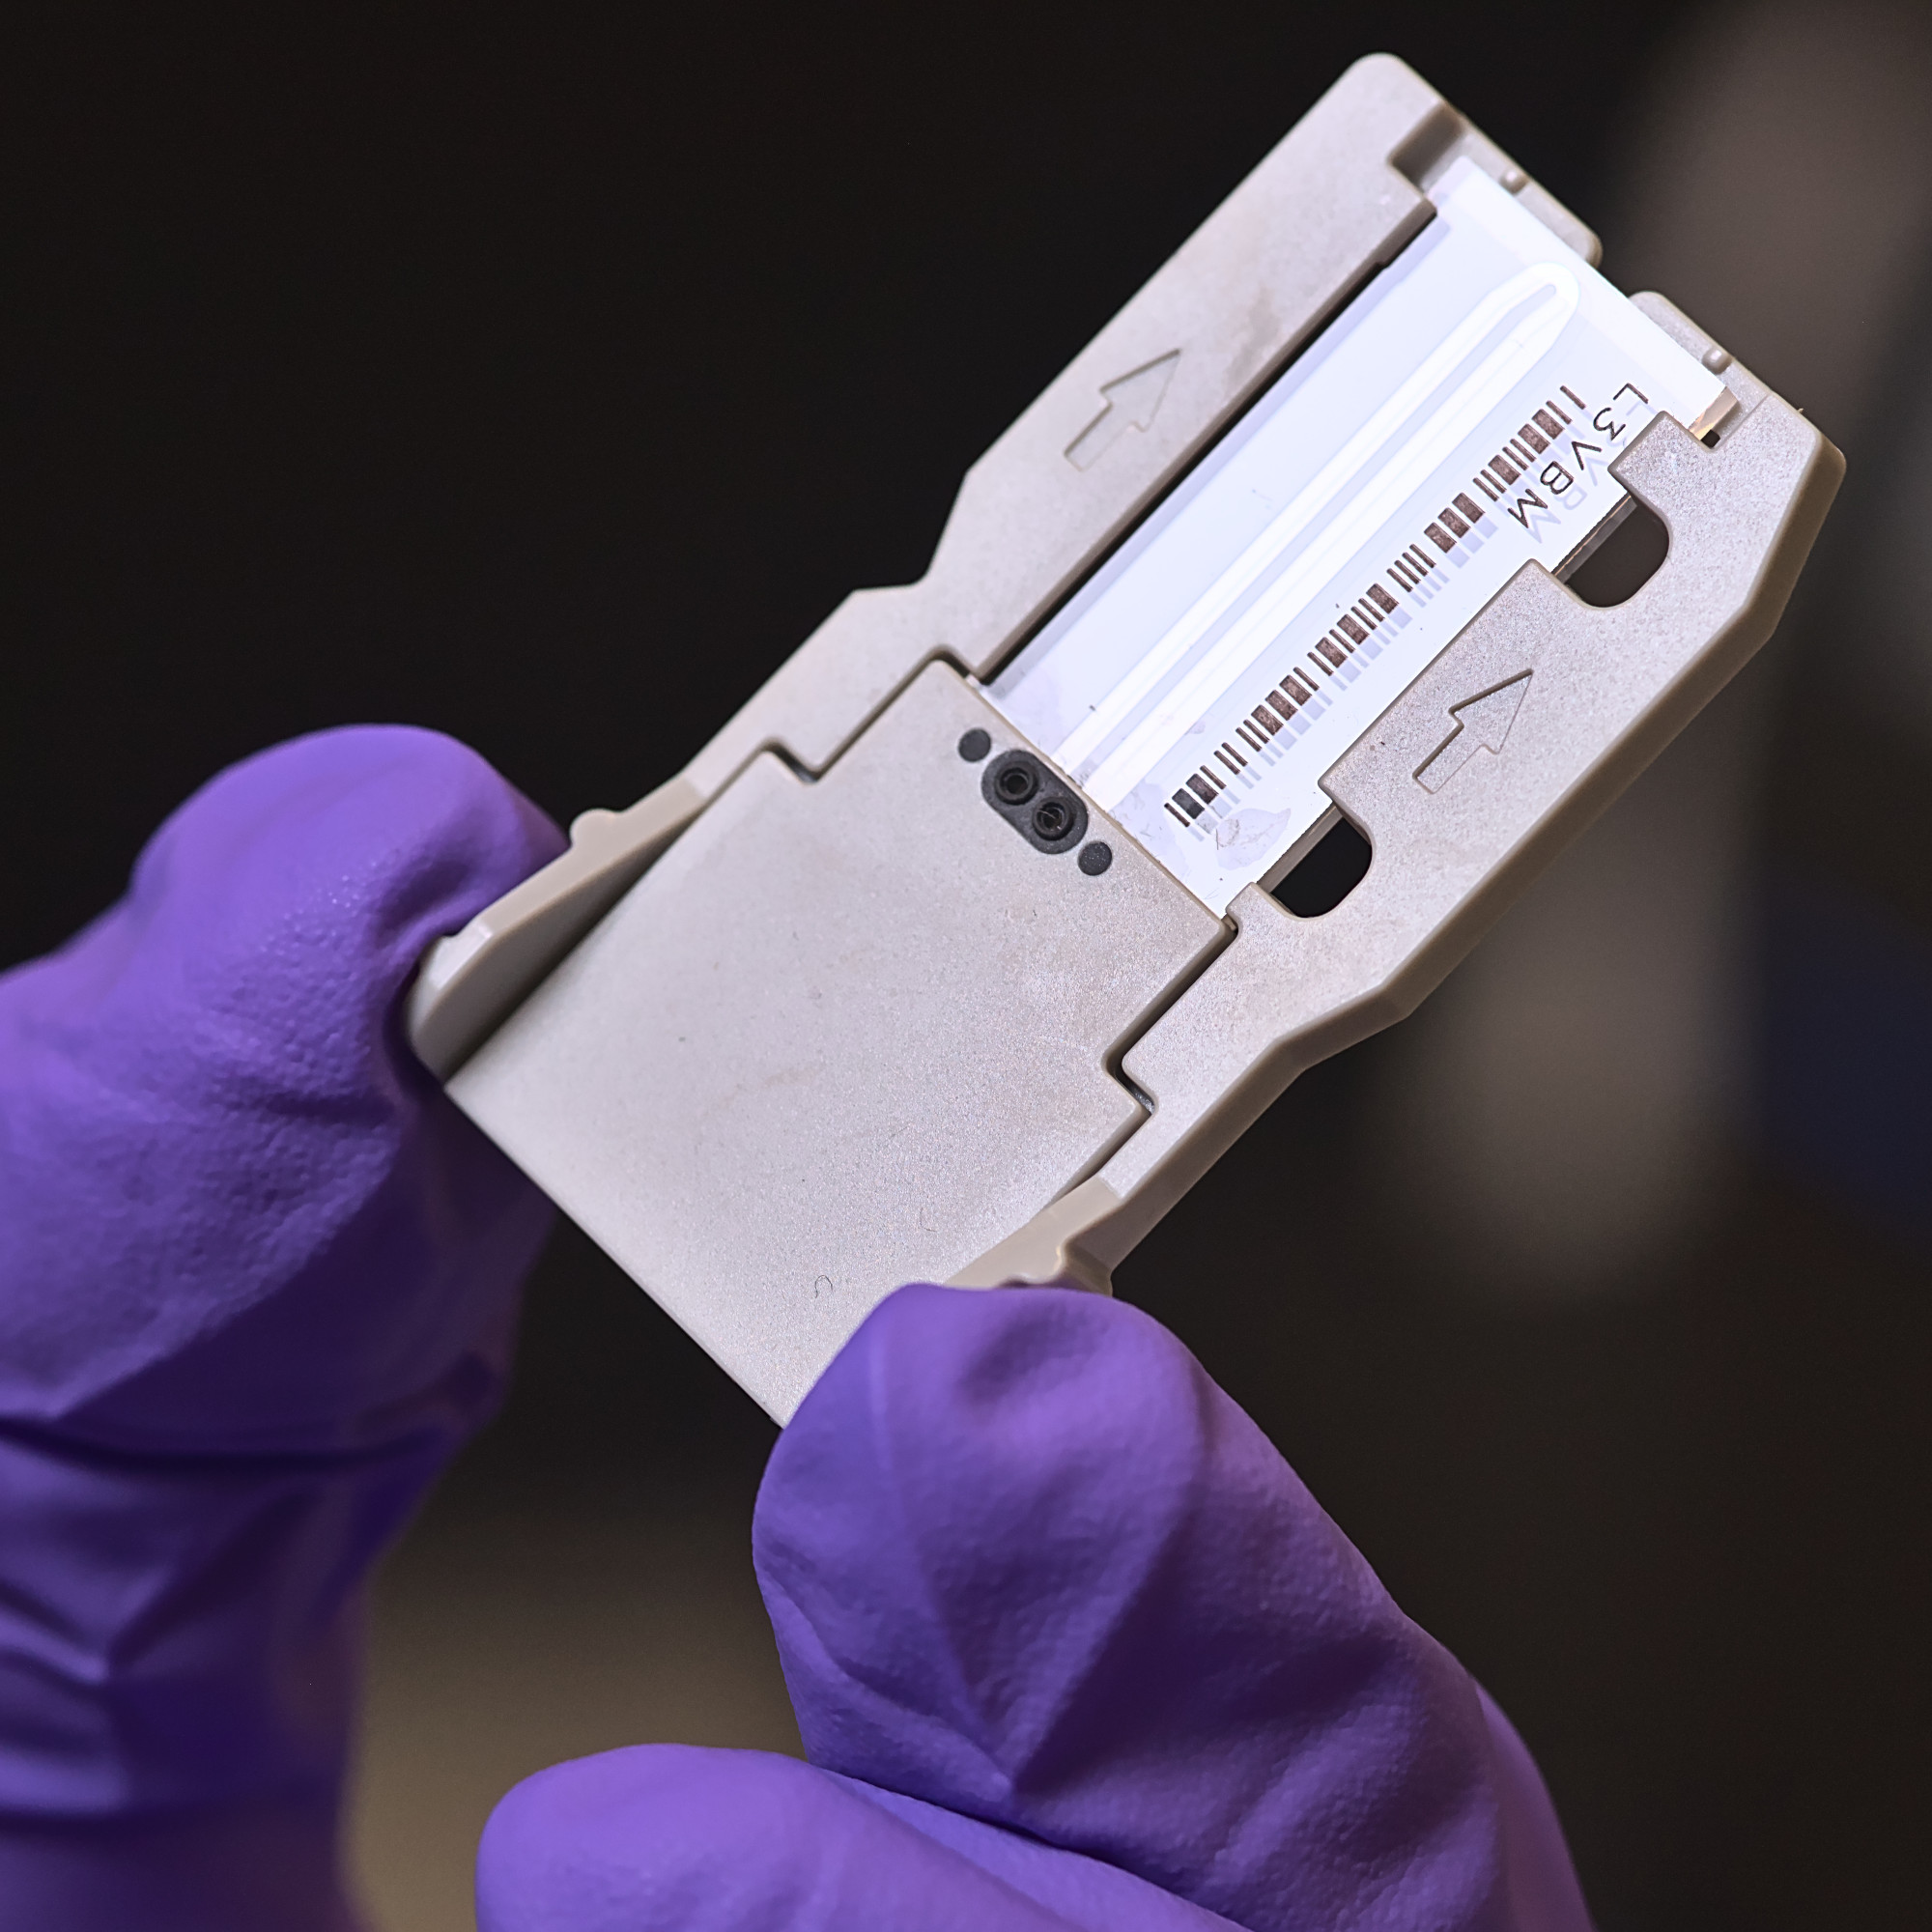
\includegraphics[width=0.24\textwidth]{./figures/flow_cell_2.jpg}
		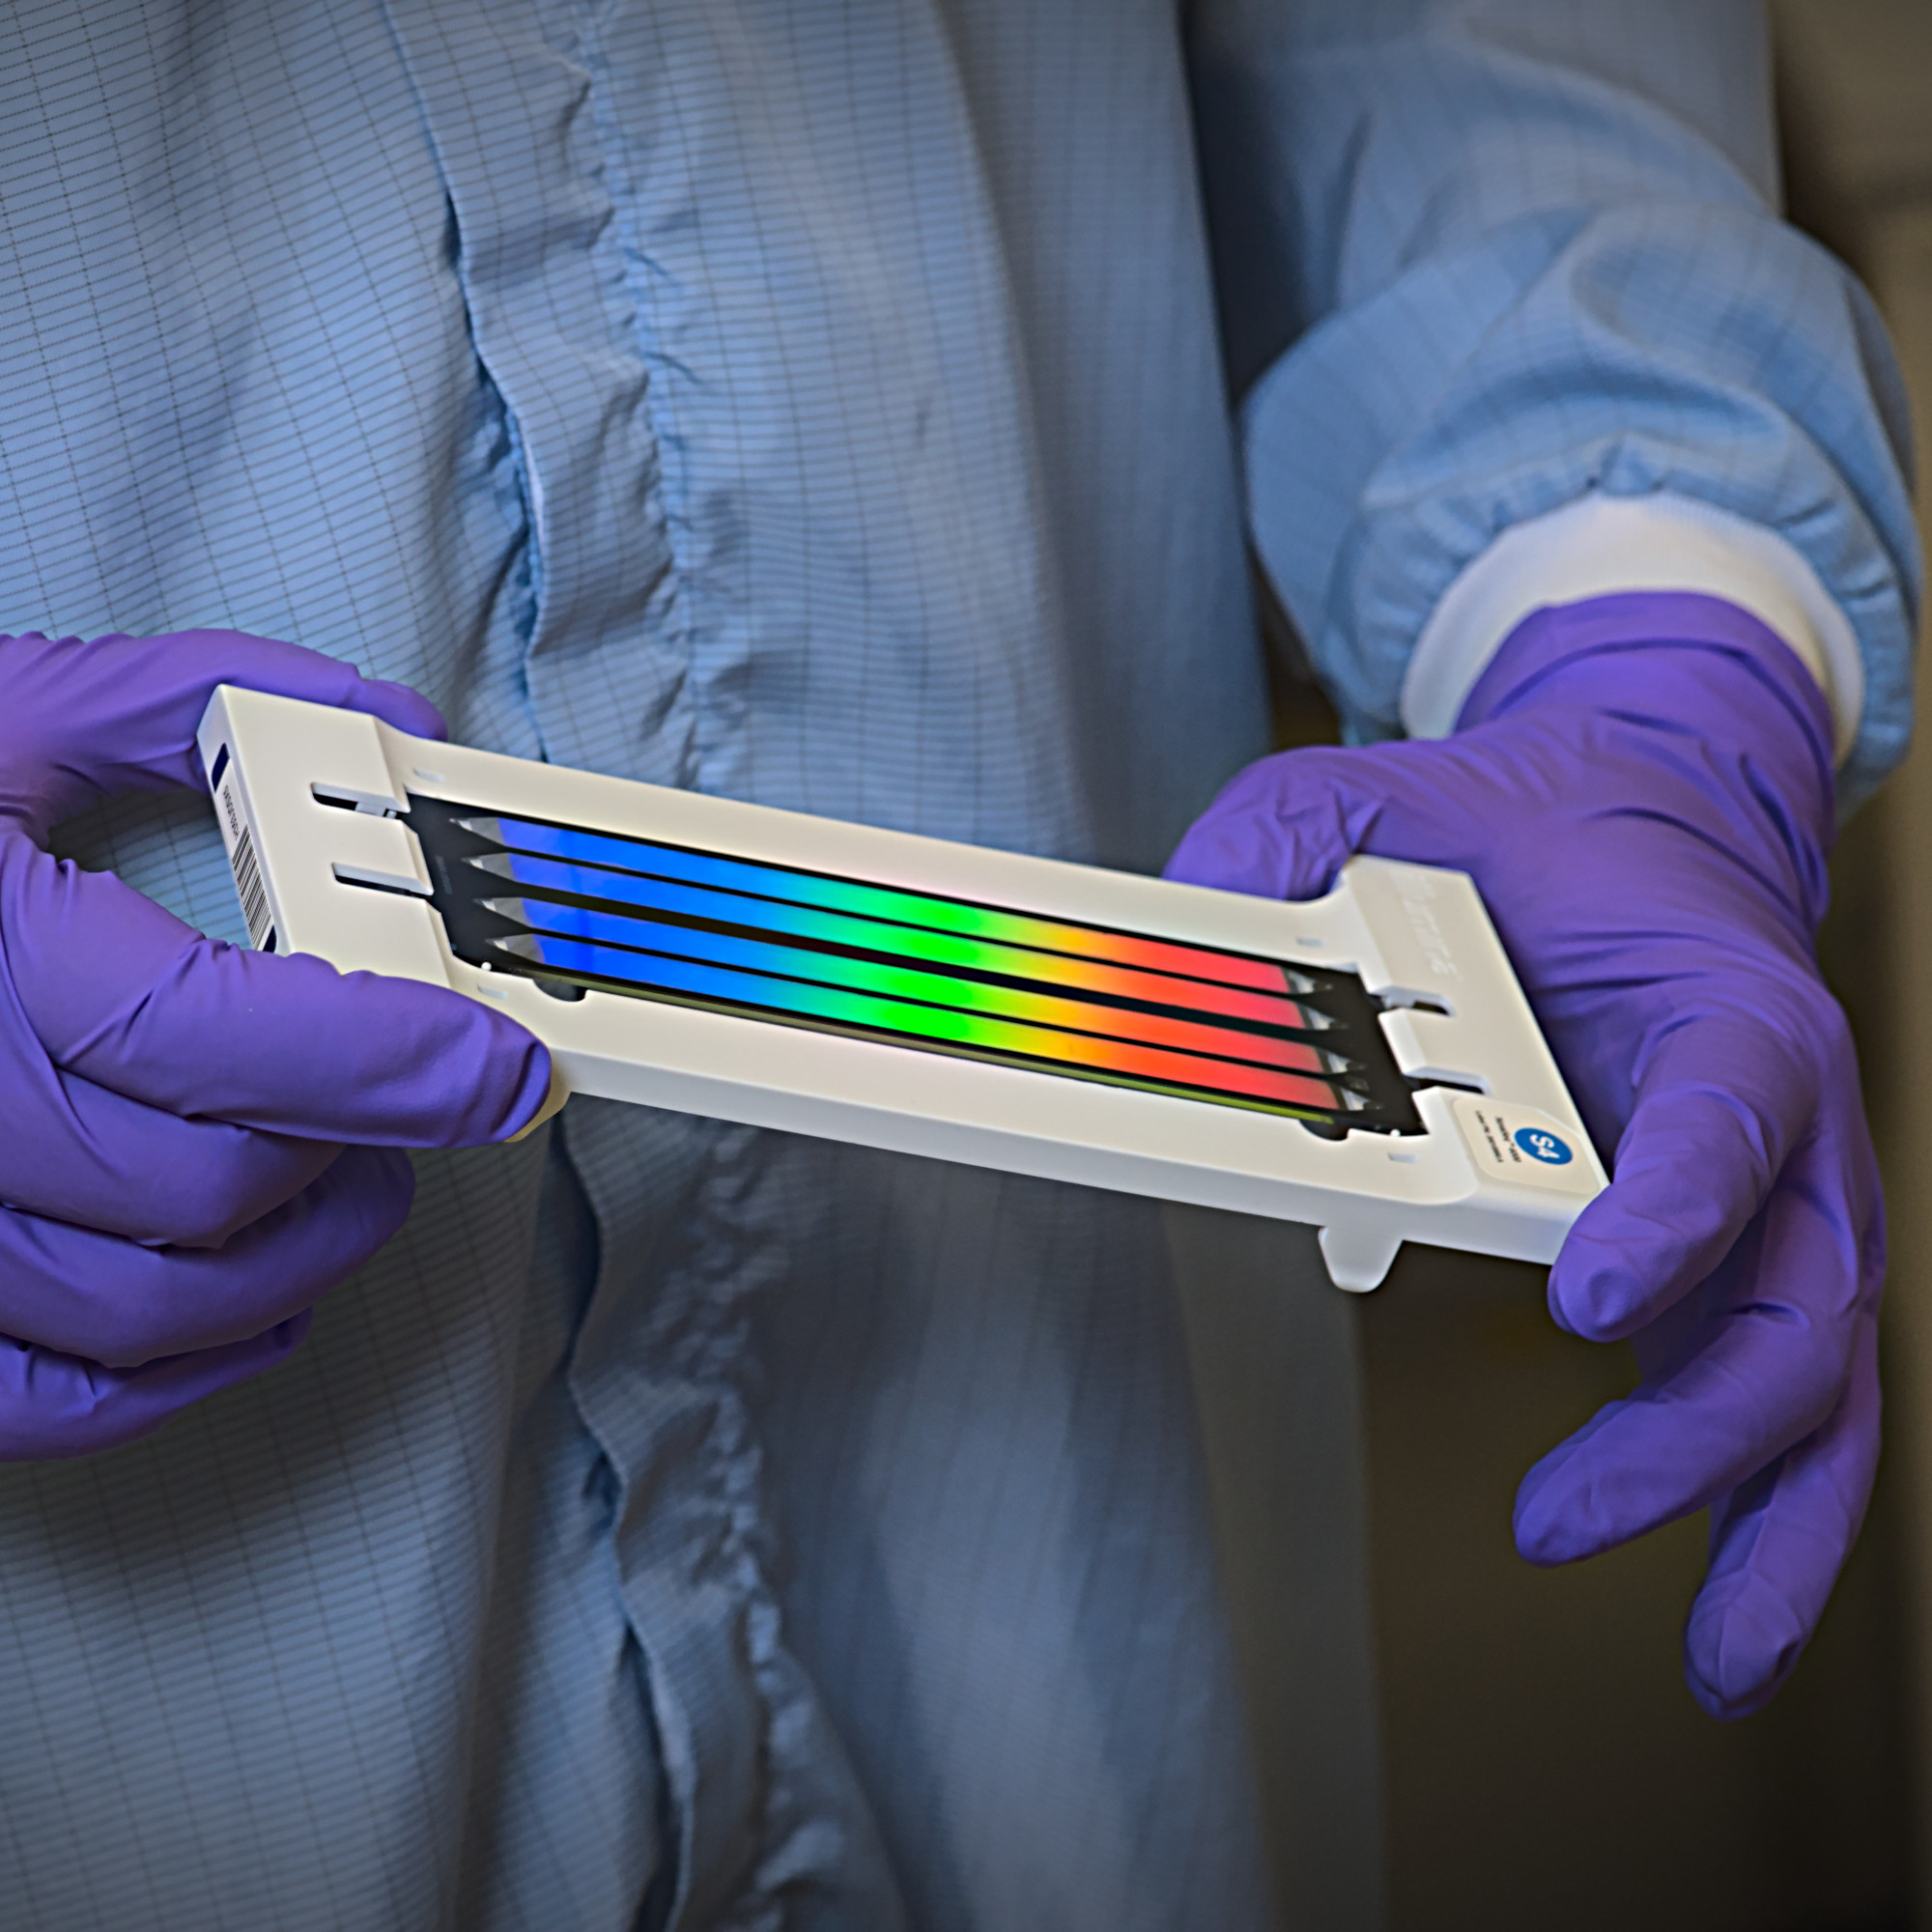
\includegraphics[width=0.24\textwidth]{./figures/flow_cell_3.jpg}
		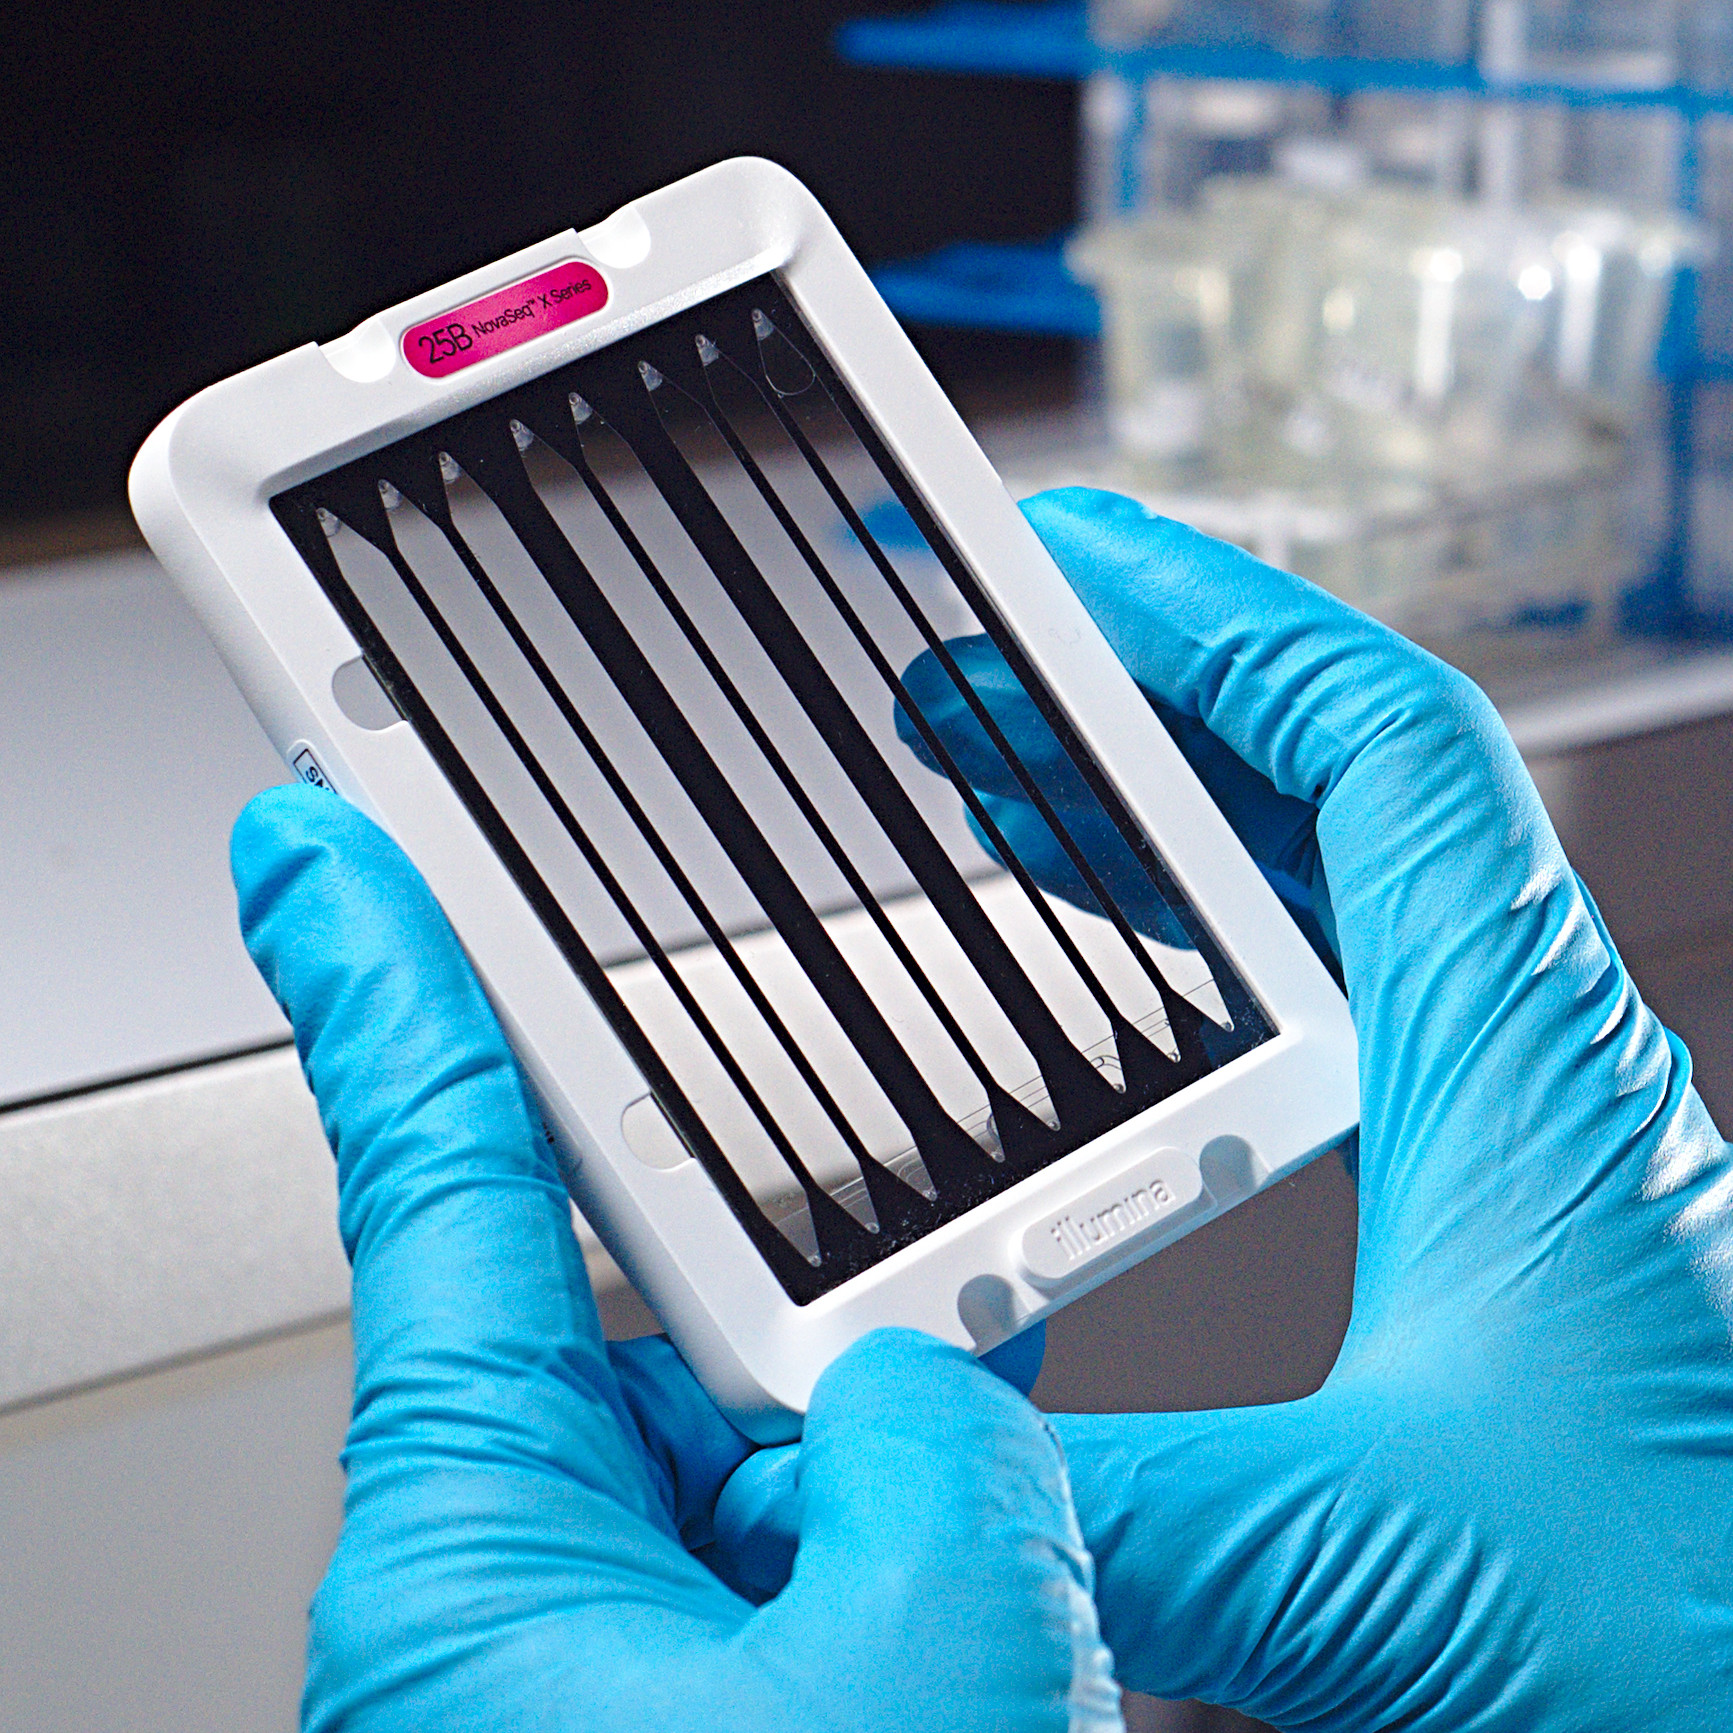
\includegraphics[width=0.24\textwidth]{./figures/flow_cell_4.jpg}
		\caption{Various Illumina flow cells}
		\end{figure}
	\end{columns}
	\begin{itemize}
		\item Illumina's platform produces 2x 150bp reads from a fragment.\linebreak\feature{$\rightarrow$ short-read sequencing}
		\item Instead of 6912 fragments like with Sanger, Illumina machines can sequence Millions to Billions in parallel \feature{$\rightarrow$ massive-parallel sequencing}
	\end{itemize}
\end{frame}

\begin{frame}{PacBio: Single-molecule sequencing by synthesis}
	\begin{columns}[T]
		\column{\dimexpr\paperwidth-10pt}
		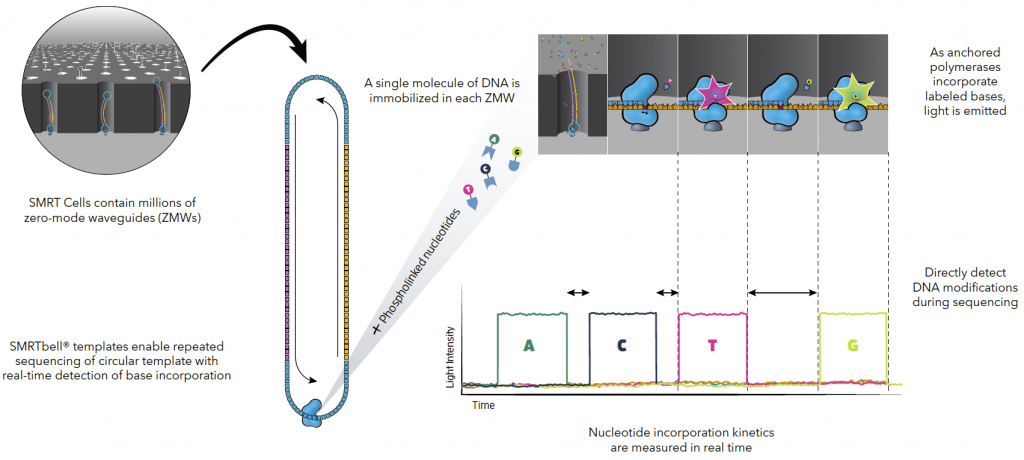
\includegraphics[width=\textwidth]{./figures/pacbio.png}
	\end{columns}
		\begin{enumerate}
			\item PacBio can generate longer reads than Illumina.
			\item Circular libraries, fragment is sequenced repeatedly.
		\end{enumerate}
\end{frame}

\begin{frame}{Oxford Nanopore: Sequencing by electric conductivity}
	\begin{columns}[T]
		\column{\dimexpr\paperwidth-10pt}
		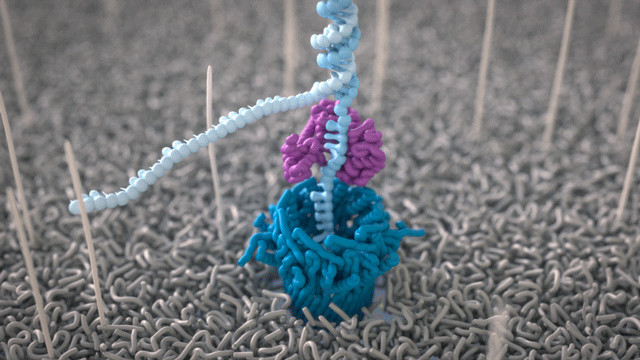
\includegraphics[width=0.493\textwidth]{./figures/MinION_GIF_06.jpg}
		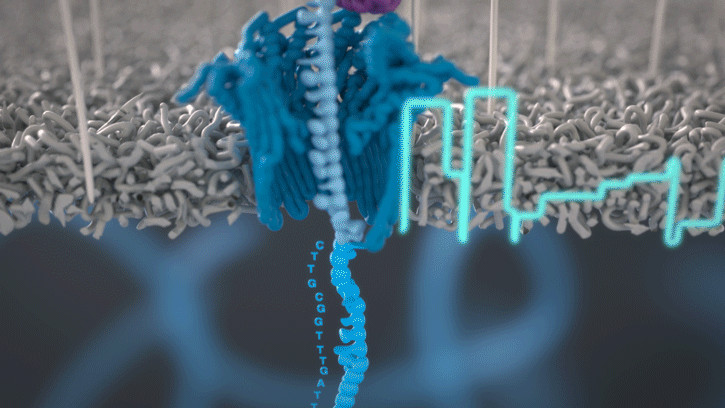
\includegraphics[width=0.493\textwidth]{./figures/MinION_GIF_08.jpg}
	\end{columns}
	\begin{columns}[T,onlytextwidth]
		\column{0.3\textwidth}
		\begin{figure}
			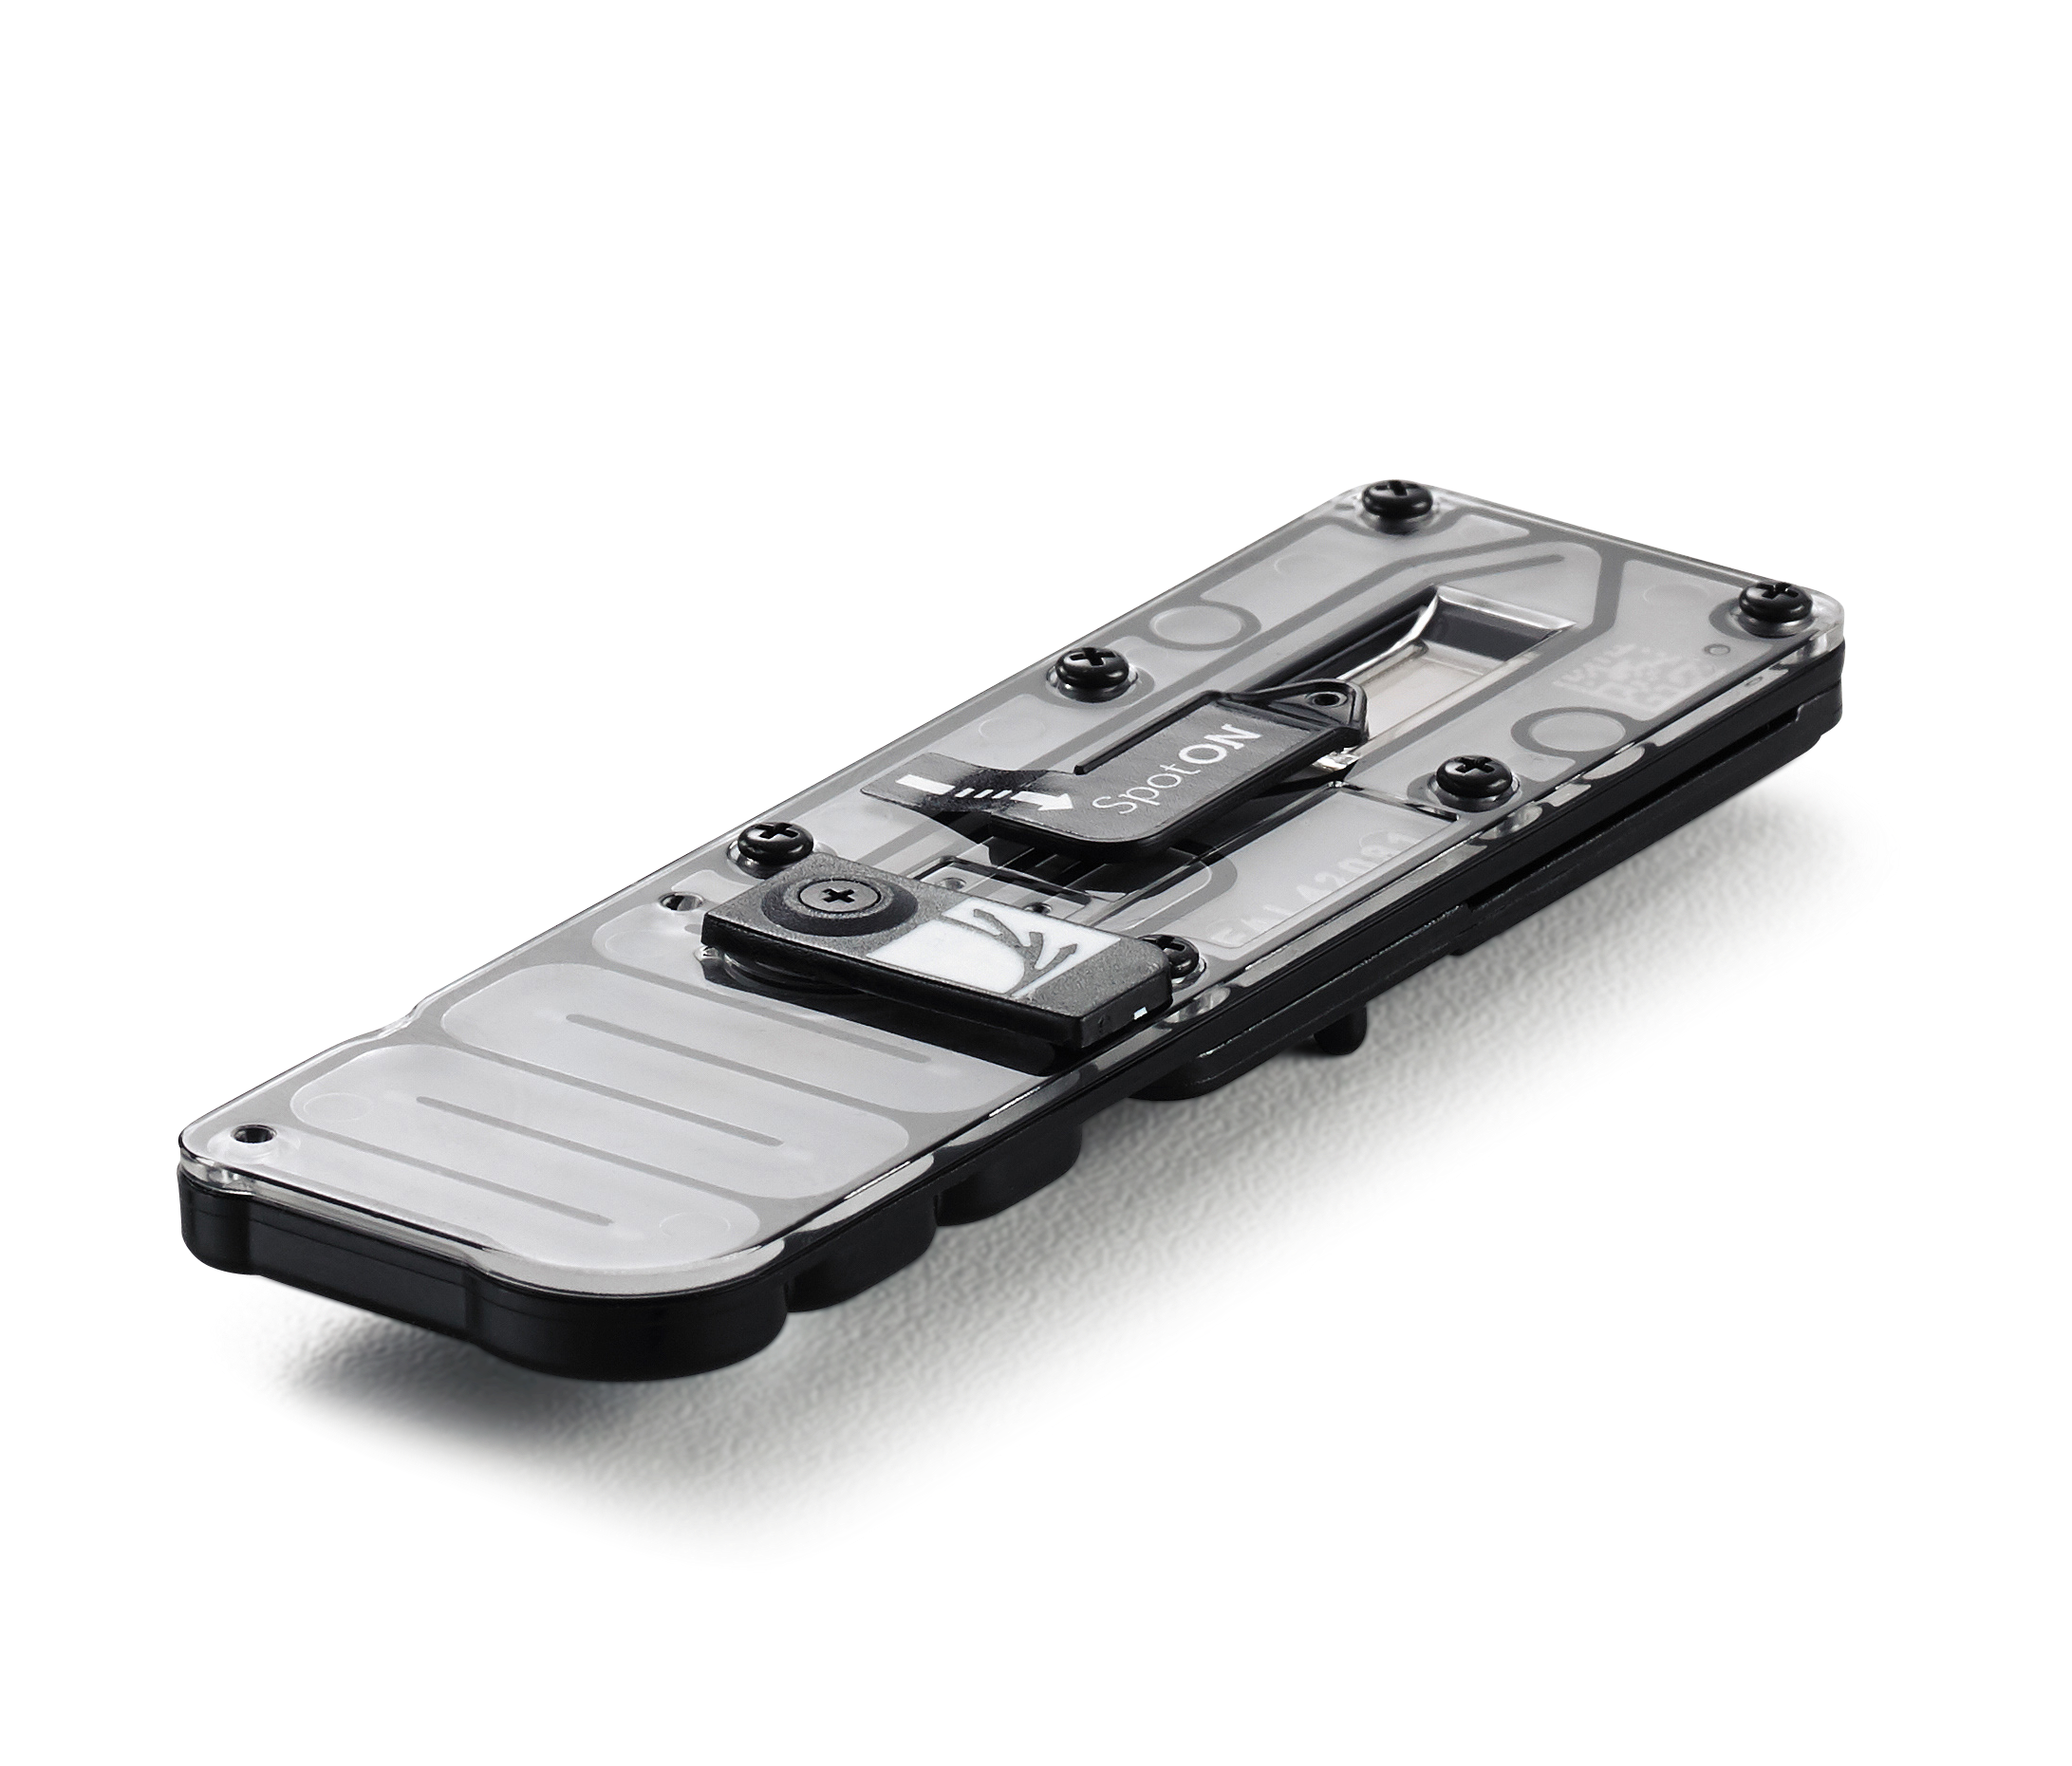
\includegraphics[width=\textwidth]{./figures/MinION Flow_Cell_transparent_3Qtr.png}
		\end{figure}
		\column{0.7\textwidth}
		\vspace{2em}
		\begin{enumerate}
			\item DNA is sequenced without amplification
			\item A motor protein pulls a DNA strand through a pore (protein channel or solid state)
			\item Bases cause specific conductivity changes
			\item Direct reading of RNA and detection of methylated bases. 
		\end{enumerate}
	\end{columns}
\end{frame}

\begin{frame}{NGI provides sequencing platforms for every need}
	%\metroset{block=fill}
	\begin{exampleblock}{Standard}
		\begin{itemize}
			\item Illumina sequencing
		\end{itemize}
	\end{exampleblock}
	\begin{alertblock}{Longer reads, less base-call errors}
	\begin{itemize}
		\item PacBio HiFi Sequencing
	\end{itemize}
\end{alertblock}
	\begin{alertblock}{Much longer reads, many more base-call errors}
	\begin{itemize}
		\item Oxford Nanopore sequencing
	\end{itemize}
\end{alertblock}
	\begin{alertblock}{Short-reads, fewest base-call errors:}
		\begin{itemize}
			\item Element Biosciences Avidite Sequencing
		\end{itemize}
	\end{alertblock}
\end{frame}

% % % % % % % % % % % % % % % % % % % % % % % 

\section{Sequencing data handling}

% % % % % % % % % % % % % % % % % % % % % % % 

\begin{frame}[fragile]{Sequencing result: Terabytes of data in FastQ-format}
	\feature{A single read:}
	\begin{enumerate}
		\item Read ID
		\item DNA-sequence
		\item +
		\item Error rate of the base call
	\end{enumerate}
	\vspace{1em}
	\hrulefill
	\vspace{1em}
\begin{columns}[T]
	\column{\dimexpr\paperwidth-10pt}
	\lstset{columns=fullflexible, basicstyle=\ttfamily,
		backgroundcolor=\color{scLGray},xleftmargin=-2.5cm,frame=lr,framesep=2pt,framerule=0pt}
		\begin{lstlisting}
			@SCILIFELAB:500:NGISTLM:1:1101:31620:1016 1:N:0
			ATAAACACGGTCTTTTTCCAGGTCAAGCCGGACGGTACCGCCCTGTGGCCATCGAA
			+
			-86<<F9FB7FFFGGGGGGFACGFFDEFGGGEFE>FGGGDGFGGFGGCFG?FF7E@
		\end{lstlisting}
\end{columns}
\end{frame}

\begin{frame}{Quality control: Good data}
	\begin{columns}[T]
		\column{\dimexpr\paperwidth-10pt}
		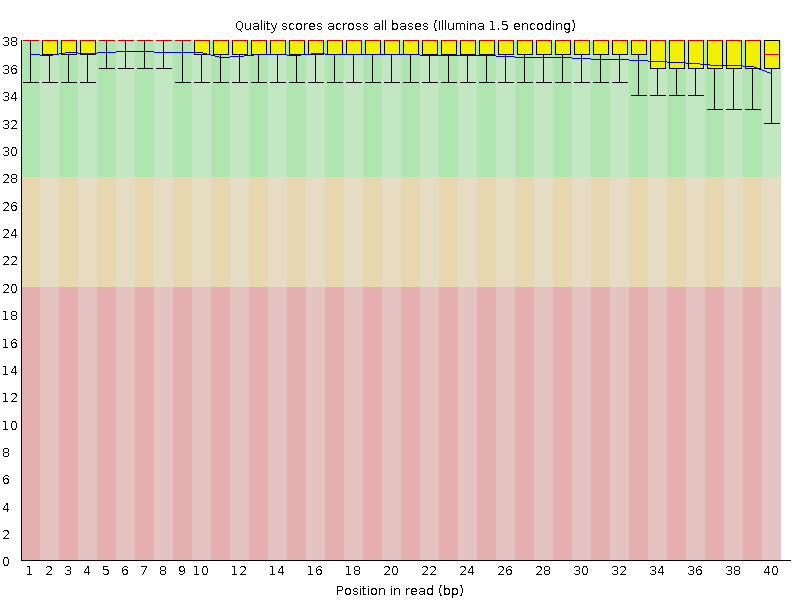
\includegraphics[width=0.493\textwidth]{./figures/fastqc-good.png}
		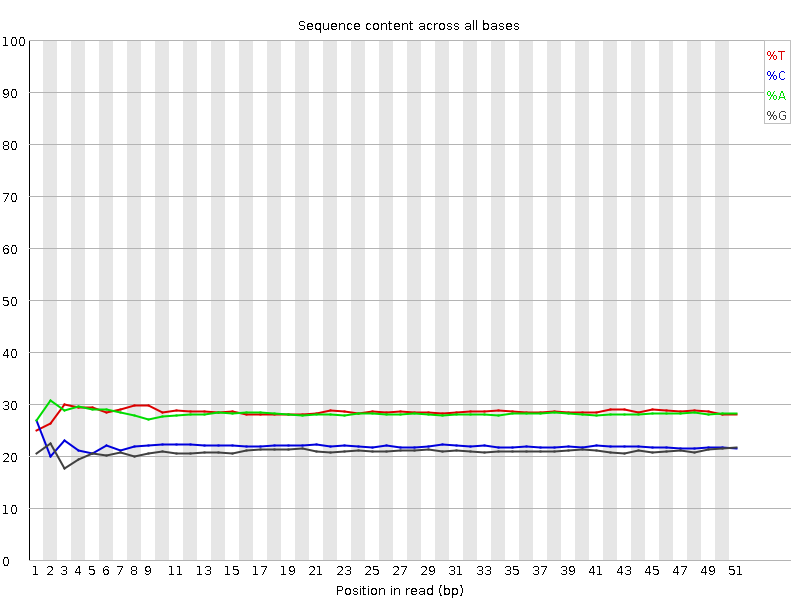
\includegraphics[width=0.493\textwidth]{./figures/fastqc-good2.png}
	\end{columns}
	\credit{\href{https://www.bioinformatics.babraham.ac.uk/projects/fastqc/}{FastQC} - A quality control tool for high throughput sequence data}
\end{frame}

\begin{frame}{Quality control: Poor data}
	\begin{columns}[T]
		\column{\dimexpr\paperwidth-10pt}
		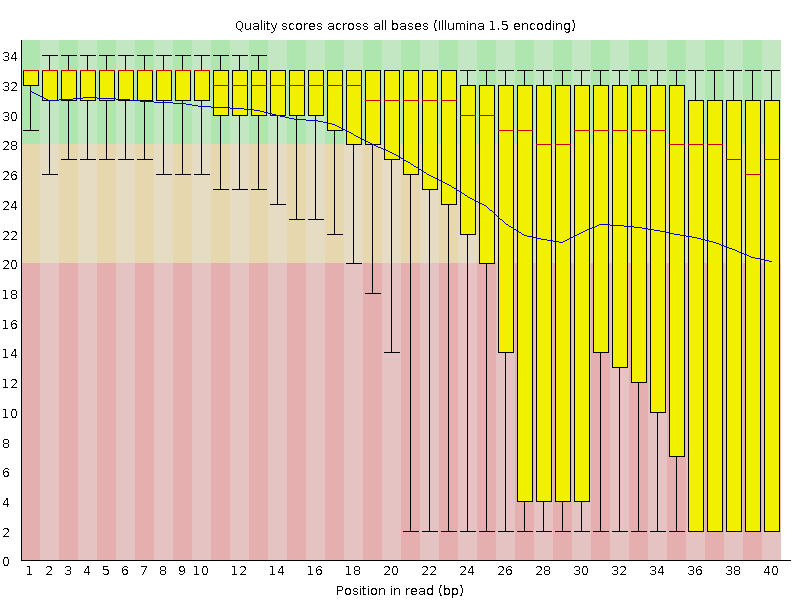
\includegraphics[width=0.493\textwidth]{./figures/fastqc-ugly.png}
		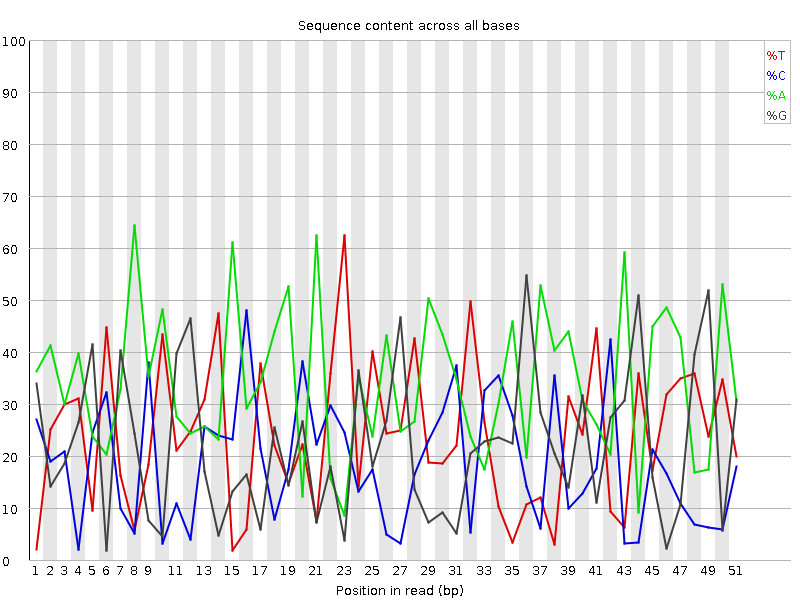
\includegraphics[width=0.493\textwidth]{./figures/fastqc-ugly2.png}
	\end{columns}
	\credit{\href{https://www.bioinformatics.babraham.ac.uk/projects/fastqc/}{FastQC} - A quality control tool for high throughput sequence data}
\end{frame}

\begin{frame}{Common bioinformatic analyses}
	\begin{columns}[T]
	\column{0.5\textwidth}
		\begin{figure}
			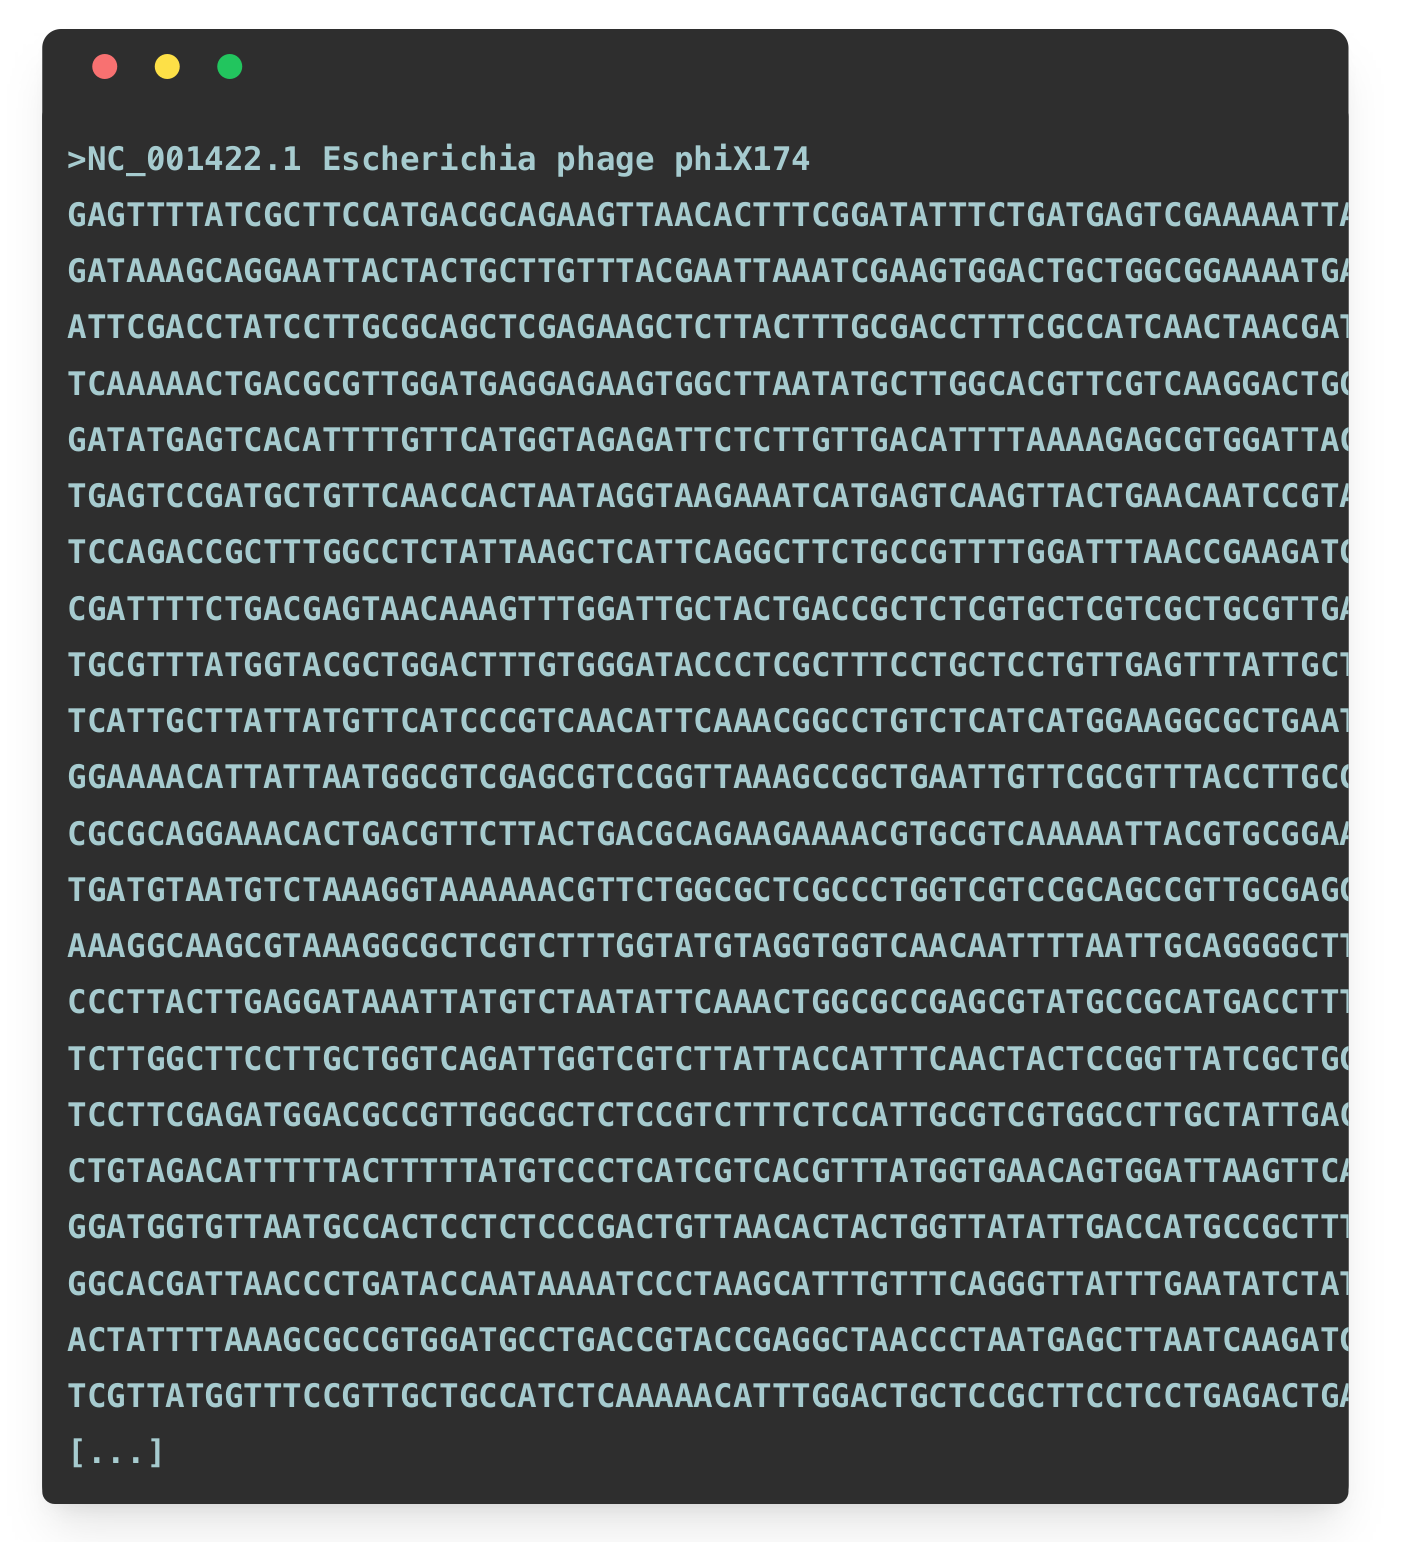
\includegraphics[width=\textwidth]{figures/phixgen.png}
		\end{figure}
		\column{0.65\textwidth}
		\vspace{1cm}
		\begin{itemize}
			\item \feature{pairwise) Alignment:} \par Find the exact origin of a short fragment in
			a long reference.
			\item \feature{Quasi-mapping:}\par Which reference is the most-likely origin?
			\item \feature{De-novo assembly:} \par Create a long reference from short
			fragments.
		\end{itemize}
	\end{columns}
\end{frame}

\begin{frame}[fragile]{Analyses as if we were back in the sixties}
	
	\begin{exampleblock}{De novo assembly of \textit{contigs} (fault-tolerant)}
		\hspace{2.3em}\framebox[1.1\width]{\small nswer, my friend} \hspace{2em}\framebox[1.1\width]{owin' in the wind. The ans} \par
		\hspace{1.35em}\framebox[1.1\width]{\small e a{\color{orange}mb}er my fr} \hfill \textbf{ Technical read error / mutation}	\par
		\hspace{5.85em}\framebox[1.1\width]{\small y friend is blowin' } \hspace{3.5em}\framebox[1.1\width]{ \small The answer is blowin' in}  \par
		\hspace{5em}\framebox[1.1\width]{\small  my friend, is blow} \hspace{2em}\framebox[1.1\width]{\small e wind. The answe}  \par
		\hspace{1.15em}\framebox[1.1\width]{\small e answer, my fr} \hspace{4.7em}\framebox[1.1\width]{\small in the wind. The answer is blowin'} \par
	\end{exampleblock}
	
	\framebox{\small The answer, my friend, is blowin' in the wind. The answer is blowin' in the wind.} 
	
	\begin{exampleblock}{Alignment (fault-tolerant)}
		\hspace{5em}\framebox[1.1\width]{\small my {\color{orange}v}riend} \hfill \textbf{Technical read error/ mutation} \par
		\framebox[1.1\width]{\small The{\color{orange}eeeeeeeee} answ{\color{orange}*}end} \hfill \textbf{Indel} \par
		\hspace{2em}\framebox[1.1\width]{\small answer} \hfill $\longleftrightarrow$ \hfill
		\framebox[1.1\width]{\small answer} \hspace{0.7em} \textbf{Multimapper} \par
	\end{exampleblock}	
\end{frame}

\begin{frame}{Analyses as if we are back today}
	\begin{columns}[T]
	\column{0.35\textwidth}
		\begin{figure}
			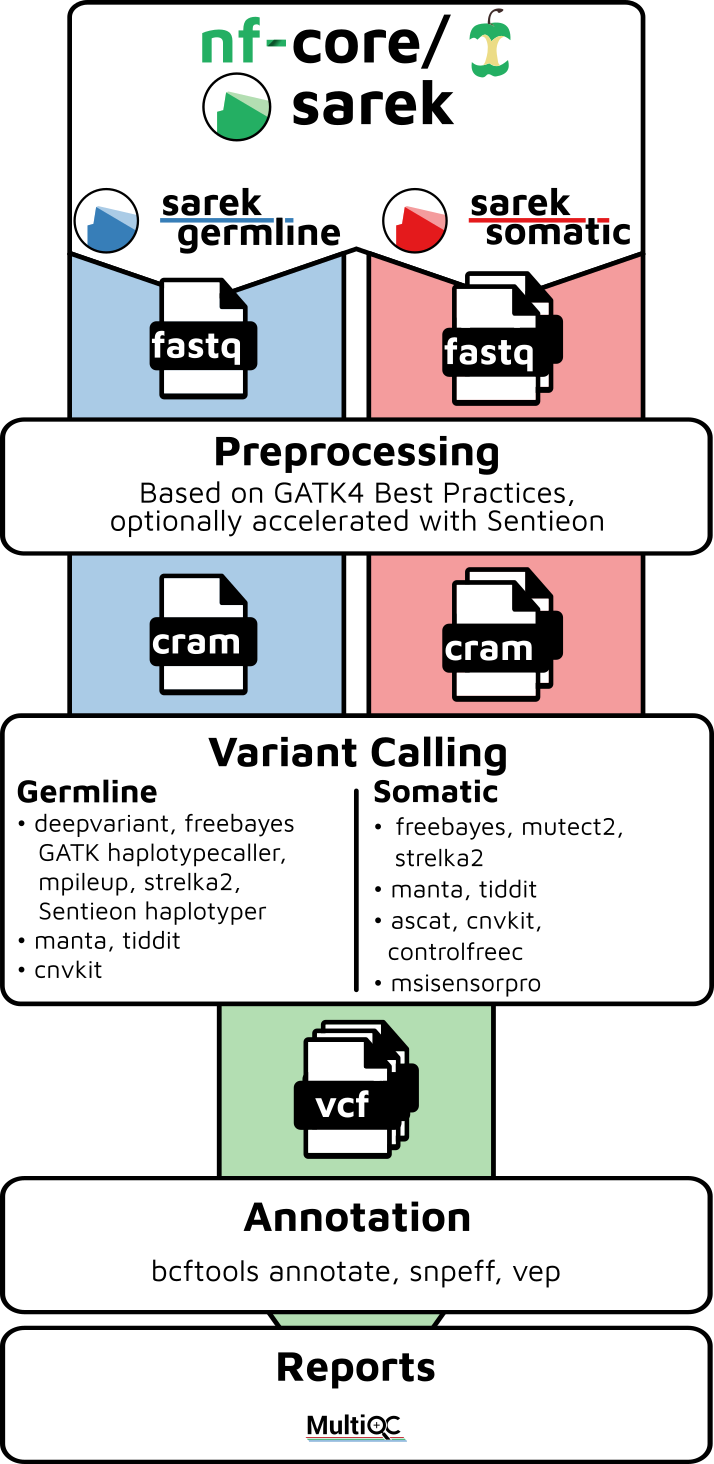
\includegraphics[width=\textwidth]{figures/sarek_workflow.png}
		\end{figure}
		\column{0.7\textwidth}
		
\includegraphics[width=0.493\textwidth]{./additional_graphics/nfcore.png}
		
\includegraphics[width=0.493\textwidth]{./additional_graphics/anvio.png}
		\begin{itemize}
			\item Data pipelines combine sequential steps.
			\item Workflow managers execute pipelines and scale analyses to many samples.
			\item Collaborative communities for workflow development help you to get started:
			\begin{itemize}
				\item \url{https://nf-co.re}
				\item \url{https://anvio.org}
			\end{itemize} 
		\end{itemize}
	\end{columns}
\end{frame}

\begin{frame}{Weblinks}
	\begin{itemize}
		\item Own lecture on NGS data analysis\linebreak \url{https://github.com/MatthiasZepper/Lecture-OmicsDataAnlysis}
		\item Course Materials on sequencing data science \linebreak \url{http://data-science-sequencing.github.io}
		\item DNA Sequencing Coursera class slides \linebreak \url{https://github.com/BenLangmead/ads1-slides}
		\item Genome Browser (Easy access to selected genomes) \linebreak \url{http://genome-euro.ucsc.edu}
		\item European Nucleotide Archive (Complete genomes and contigs) \linebreak \url{https://www.ebi.ac.uk/ena}
		\item Current human reference genome (version 38) \linebreak \url{http://ncbi.nlm.nih.gov/projects/genome/assembly/grc/human/}
	\end{itemize}
\end{frame}




% % % % % % % % % % % % % % % % % % % % % % % 

\section{Sequencing applications}

% % % % % % % % % % % % % % % % % % % % % % % 

\begin{frame}{We are surrounded by genetic information}
	\begin{columns}[T]
		\column{\dimexpr\paperwidth-10pt}
		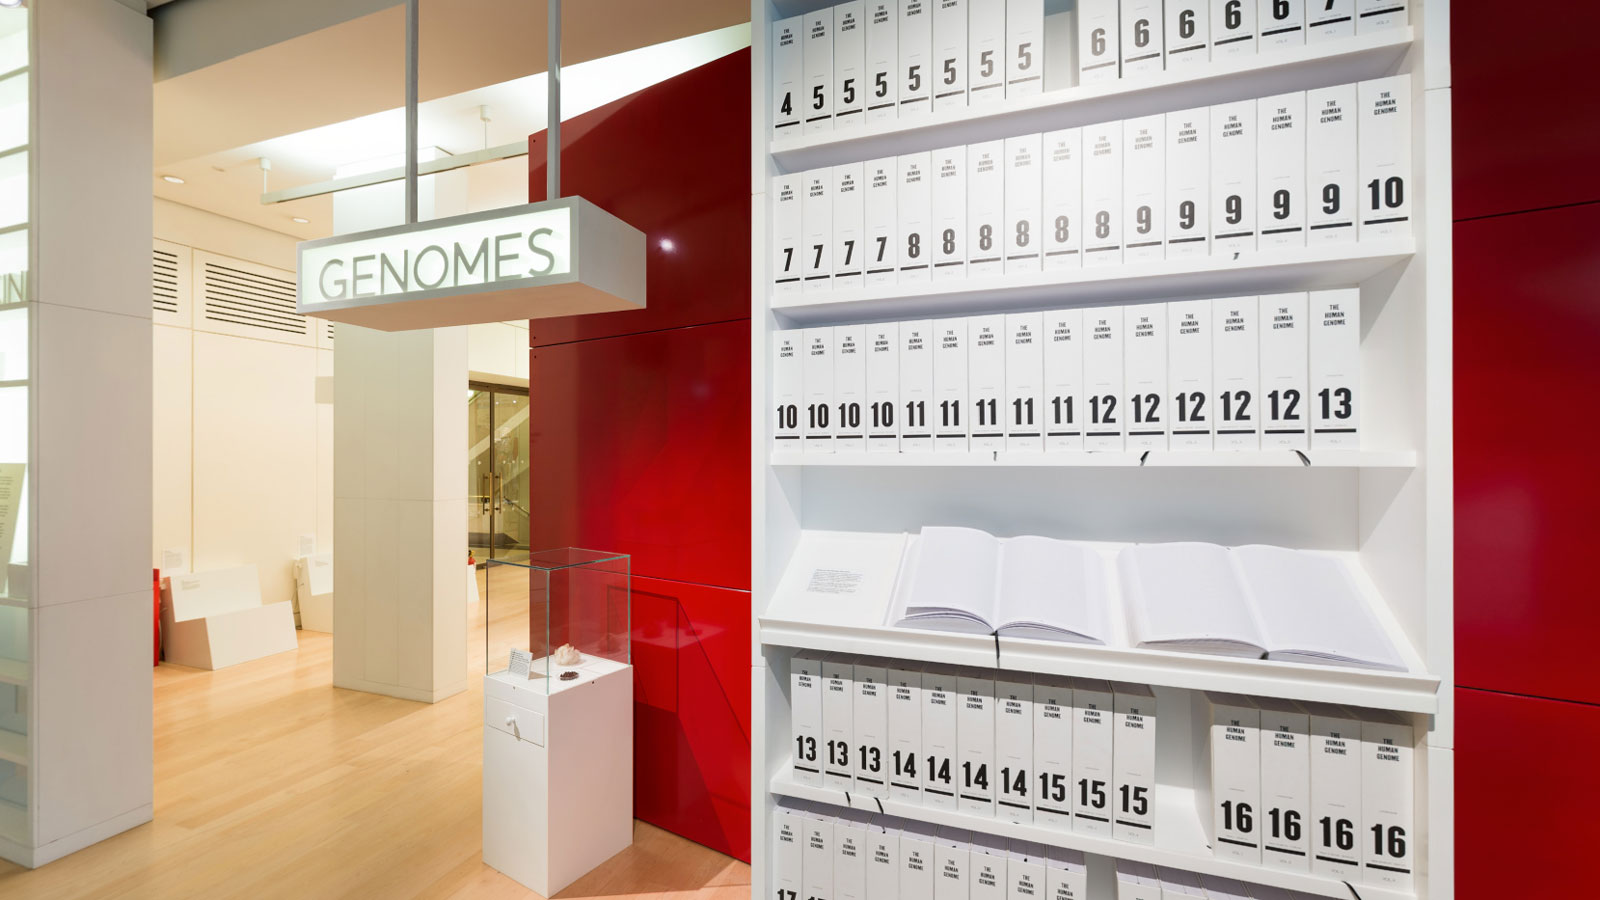
\includegraphics[width=\textwidth]{./figures/WellcomeCollectionGenome.jpg}
	\end{columns}
\credit{Library of the Human Genome, Wellcome Collection. Photo by Ben Gilbert and Thomas Farnetti}
\end{frame}

\begin{frame}{We are surrounded by genetic information: Many applications}
	\begin{columns}[T]
		\column{\dimexpr\paperwidth-10pt}
		
\includegraphics[width=\textwidth]{./figures/WellcomeCollectionGenomePapers.png}
	\end{columns}
\end{frame}

\begin{frame}{Not a finite list, but let's tidy up}
	\begin{exampleblock}{Applications that characterize genetic (mal)function}
		\begin{itemize}
			\item Gene expression / Transcriptomics (RNA-seq, CAGE-seq)
			\item Gene regulation / Epigenetics (DNA-Methylation, Histone modifications)
			\item Gene alterations (Hereditary diseases, cancer biology)
		\end{itemize}
	\end{exampleblock}
	\begin{exampleblock}{Applications that explore what is around us}
		\begin{itemize}
			\item Genome assemblies of other species (biodiversity)
			\item Metagenomics (environmental DNA)
			\item Pathogen surveillance (antibiotic resistance, epidemics)
		\end{itemize}
	\end{exampleblock}
	\begin{exampleblock}{Applications to elucidate evolutionary processes}
	\begin{itemize}
		\item Ancient genomes
		\item Population genomics
	\end{itemize}
\end{exampleblock}
\end{frame}

\begin{frame}[standout]{}
	
\includegraphics[width=0.6\textwidth]{./figures/onedoesnotsimplyB2.jpg} \par \vspace{1cm} \par
	{\normalsize \feature{Sequencing application:} Combination of a library preparation method and a suitable sequencing technology}
\end{frame}

% % % % % % % % % % % % % % % % % % % % % % % 

\section{Applications that characterize genetic (mal)function}

% % % % % % % % % % % % % % % % % % % % % % % 

\begin{frame}[fragile]{Epigenetics: Regulatory layers of the genome}
	\begin{columns}
		\column{0.5\textwidth}
		
		Cells of an organism contain the identical genome but utilize it in different ways.
		
		\column{0.5\textwidth}
		\vspace{2em} \\ \hfill 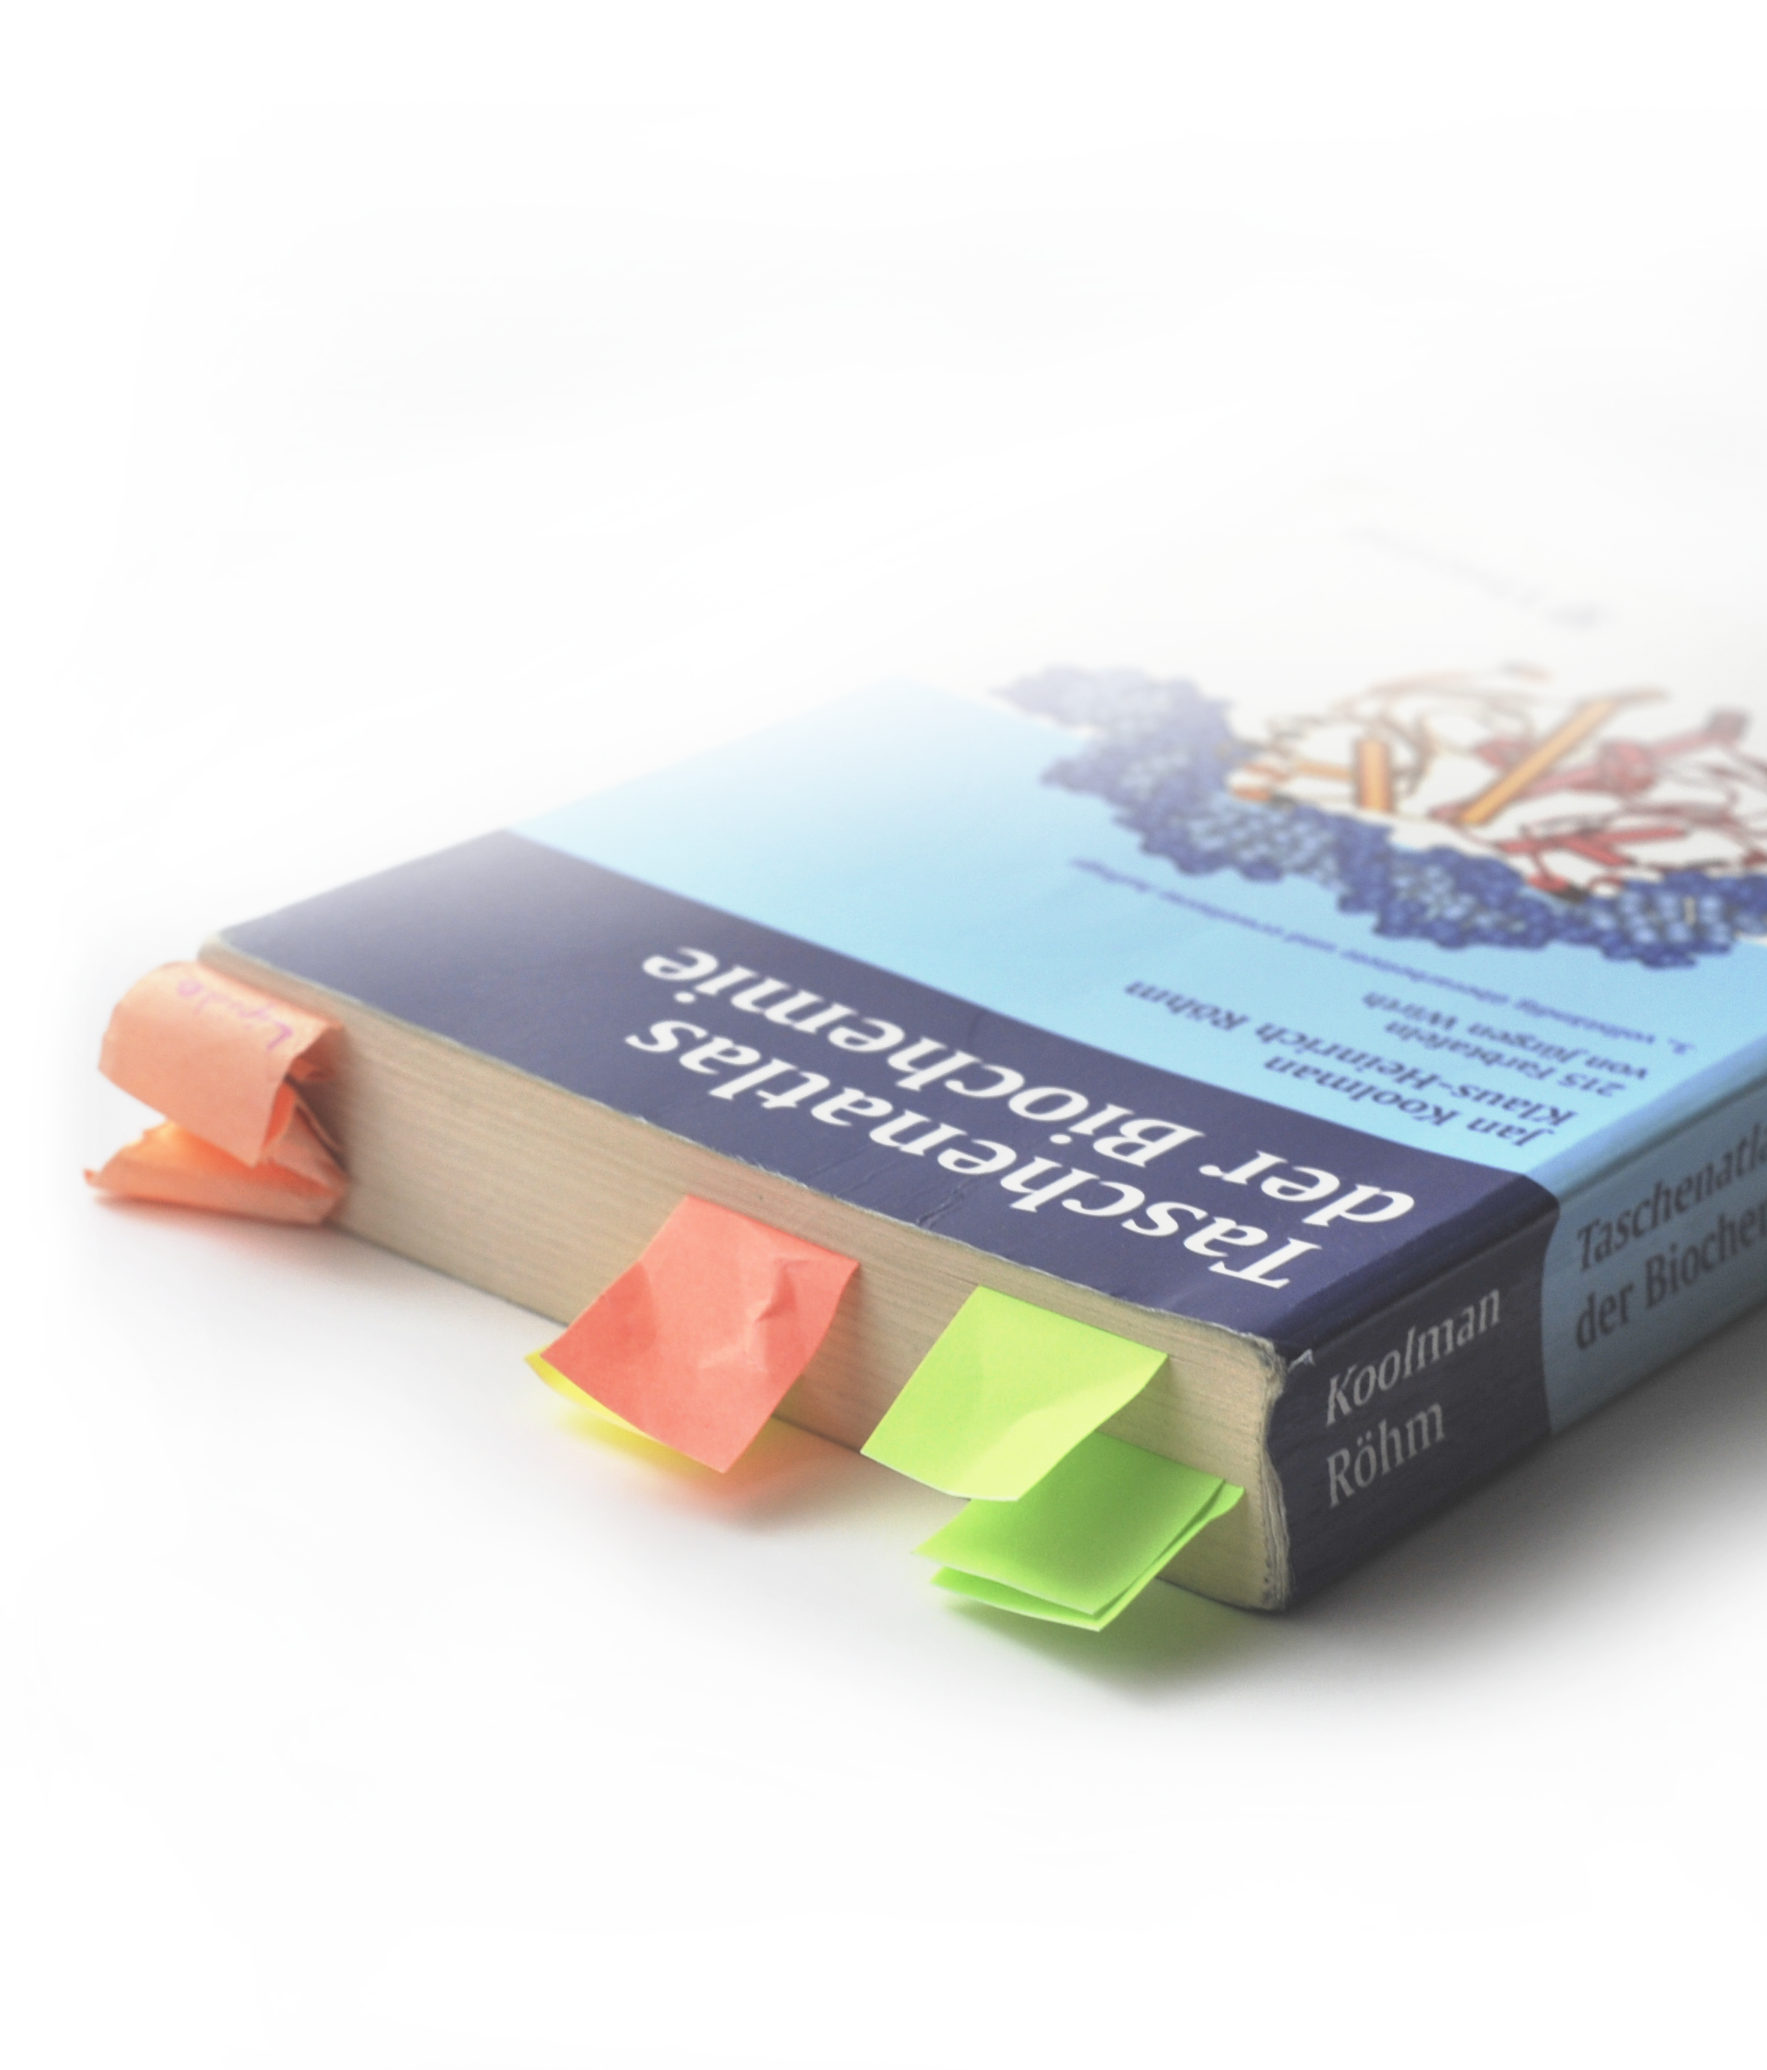
\includegraphics[height=0.8\textheight]{./figures/lesezeichen.png} 
	\end{columns}
\end{frame}

\begin{frame}{ChIP-seq: \underline{Ch}romatin \underline{I}mmuno\underline{p}recipitation \underline{Seq}uencing}
	\begin{minipage}{.46\linewidth}
		\begin{center}
			{\resizebox{\textwidth}{!}{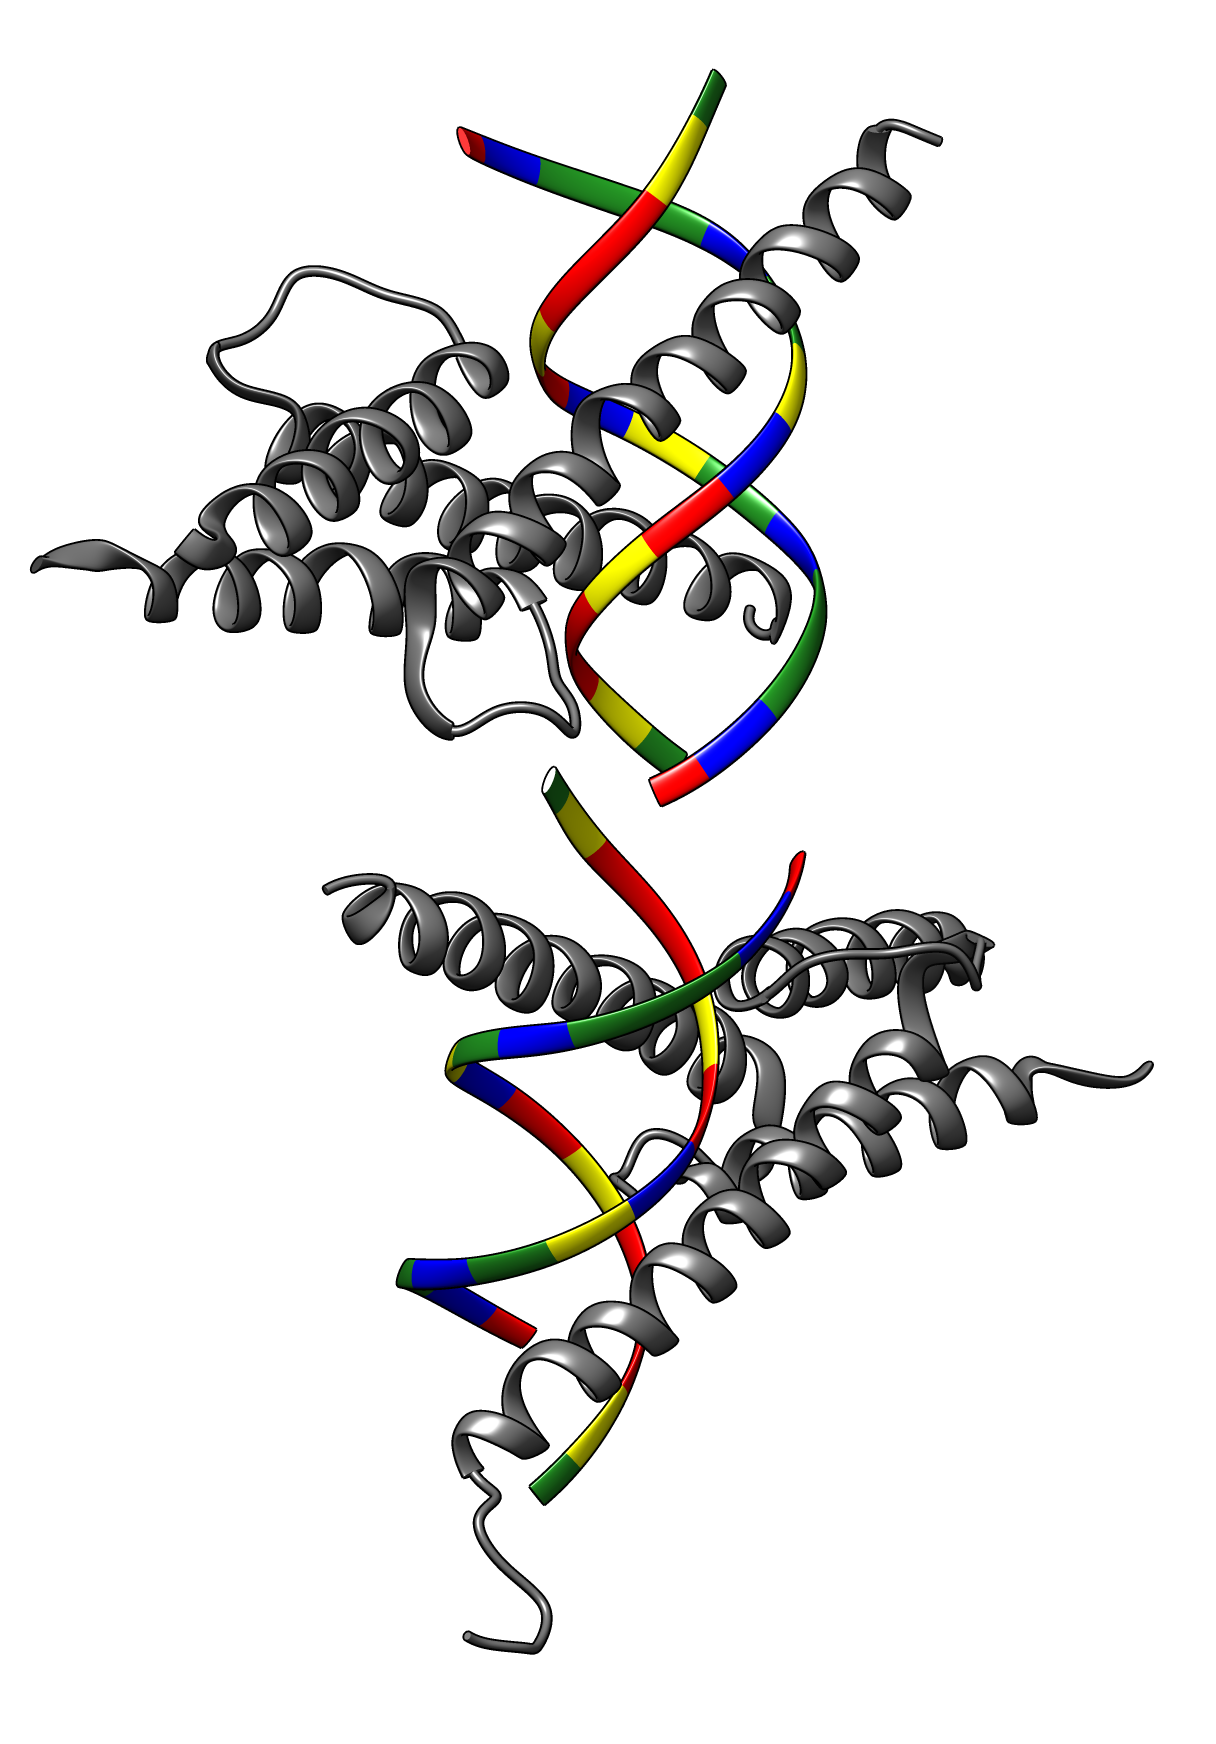
\includegraphics{./figures/helixloophelix.png}}}
		\end{center}
	\end{minipage}
	%\hspace{0.1\linewidth}
	\begin{minipage}{.53\linewidth}
		\begin{itemize}
			\item Which genomic sites are bound by a particular protein?
			\item Can detect transcription factor binding or epigenetic histone modifications.
		\end{itemize}
		\vspace{2em}
		{\begin{flushleft}
				\scriptsize $\leftarrow$ Two HLH-motifs (grey) of the  helix-loop-helix-transcription factor MyoD are bound to DNA.\end{flushleft}}
	\end{minipage}%
	\credit{\begin{flushleft}
			\url{https://www.ebi.ac.uk/pdbe/entry/pdb/1mdy} \linebreak Rendering with \href{http://www.cgl.ucsf.edu/chimera}{UCSF Chimera} \end{flushleft}}
\end{frame}

\begin{frame}{ChIP-seq: \underline{Ch}romatin \underline{I}mmuno\underline{p}recipitation \underline{Seq}uencing}
	\vspace{3em}
	\begin{center}
		\includegraphics[width=\textwidth]{./figures/ChIPseq1.png}
	\end{center}
	\begin{minipage}[t]{.49\linewidth}
		\begin{enumerate}
			\item {Isolation of target cells}
		\end{enumerate}
	\end{minipage}
	\begin{minipage}[t]{.49\linewidth}
		\begin{enumerate}
			\stepcounter{enumi}
			\item { \textit{Cross-linking:} Stably bind proteins to DNA with covalent bonds}
		\end{enumerate}
	\end{minipage}
	\credit{Fig: own derivative work. Original: \href{http://commons.wikimedia.org/wiki/File:Chromatin\_immunoprecipitation\_sequencing.svg}{Jon Chui, Wikimedia Commons, CC-BY-SA 3.0}}
\end{frame}

\begin{frame}{ChIP-seq: \underline{Ch}romatin \underline{I}mmuno\underline{p}recipitation \underline{Seq}uencing}
	\vspace{3em}
	\begin{center}
		\includegraphics[width=\textwidth]{./figures/ChIPseq2.png}
	\end{center}
	\begin{minipage}[t]{.49\linewidth}
		\begin{enumerate}
			\setcounter{enumi}{2}
			\item \textit{Lysis + Sonication}: Lyse cells and fragment DNA by ultrasonic sound
		\end{enumerate}
	\end{minipage}
	\begin{minipage}[t]{.49\linewidth}
		\begin{enumerate}
			\setcounter{enumi}{3}
			\item \textit{Precipitation}: Recover target protein and bound DNA from lysate
			% Antikörper gekoppelt an  Agarose, Sepharose or Magnetische Kügelchen
		\end{enumerate}
	\end{minipage}
	\credit{Fig: own derivative work. Original: \href{http://commons.wikimedia.org/wiki/File:Chromatin\_immunoprecipitation\_sequencing.svg}{Jon Chui, Wikimedia Commons, CC-BY-SA 3.0}}
\end{frame}

\begin{frame}{ChIP-seq: \underline{Ch}romatin \underline{I}mmuno\underline{p}recipitation \underline{Seq}uencing}
	\begin{enumerate}
		\setcounter{enumi}{4}
		\item Decrosslink and recover formerly bound DNA
		\item Sequence DNA
		\item Alignment on the reference genome
	\end{enumerate}
	\begin{center}
		\includegraphics[width=\textwidth]{./figures/igvpeaks.png}
	\end{center}
	\begin{enumerate}
		\setcounter{enumi}{7}
		\item Subtract signals from negative control (IgG-control)
		\item Peak detection and assignment to genes
	\end{enumerate}
	\credit{Screenshot \href{https://igv.org/doc/desktop/}{Integrative Genomics Viewer (IGV)}}
\end{frame}

\begin{frame}{Peaks of different applications: Histone ChIP-seq, RNA-seq,  CAGE-seq}
	\begin{columns}[T]
		\column{\dimexpr\paperwidth-10pt}
		\includegraphics[width=\textwidth]{./figures/peaks.png}
	\end{columns}
\end{frame}

\begin{frame}{Big sequencing projects addressed basic research on gene regulation}
	\begin{center}
		\includegraphics[width=0.9\textwidth]{./figures/EncodeNatureGraphic.png}
	\end{center}
    \begin{itemize}
    	\item \href{https://www.encodeproject.org}{ENCODE Project: ENCyclopedia Of DNA Elements}
    	\item \href{http://www.cell.com/consortium/IHEC}{Int. Human Epigenome Consortium}
    \end{itemize}
	\credit{Fig.: Darryl Leja (NHGRI), Ian Dunham (EBI)}
\end{frame}

\begin{frame}{Most methods now on single-cell level}
	\begin{columns}[T]
		\column{\dimexpr\paperwidth-10pt}
		\begin{figure}
			\includegraphics[width=0.24\textwidth]{./figures/single-cell-B-oil.png}
			\includegraphics[width=0.24\textwidth]{./figures/single-cell-B-oil2.png}
			\includegraphics[width=0.24\textwidth]{./figures/single-cell-B-oil3.png}
			\includegraphics[width=0.24\textwidth]{./figures/single-cell-B-oil4.png}
			\caption{Artificial DNA barcode tags allow to determine cell of origin}
		\end{figure}
	\end{columns}
	\begin{figure}
		\includegraphics[width=0.9\textwidth]{./figures/single-cell4.png}
		\caption{Dimensionality reduction methods (UMAP, t-SNE) separate cell-types}
	\end{figure}
	\credit{Figures by Anja Mezger}
\end{frame}

\begin{frame}{Spatial transcriptomics: Microscopy + single-cell sequencing}
	\begin{figure}
		\includegraphics[width=0.9\textwidth]{./figures/10x2.png}
		\caption{Cell barcodes on microscopy slide}
	\end{figure}
\end{frame}

\begin{frame}{Spatial transcriptomics: Microscopy + single-cell sequencing}
	\begin{center}
		\includegraphics[width=\textwidth]{./figures/hca.png} \\
	\end{center}
	\url{https://www.humancellatlas.org}
	\credit{\citeme{Wang2018}, Science 361(6400)}
\end{frame}

\begin{frame}{SciLifeLab is one of the birthplaces of spatial transcriptomics}
	\begin{center}
		\includegraphics[width=\textwidth]{./figures/visium10x.png} \\
	\end{center}
	\url{https://www.spatialresearch.org}
\end{frame}

\begin{frame}{Cancer cell genomes (Recurrent mutations and aberrations)}
	\begin{columns}
		\begin{column}{0.3\textwidth}
			\begin{itemize}
				\item  Cancer Genome Project 
				\item  Cancer Genome Atlas 
				\item  PanCanAtlas
				\item $\cdots$
			\end{itemize}
		\end{column}
		\begin{column}{0.7\textwidth}
			\begin{center}
				\includegraphics[width=\textwidth]{./figures/canceraltsplicing.png}
			\end{center}
			\begin{center}
				\includegraphics[width=\textwidth]{./figures/p53.png}
			\end{center}
		\end{column}
	\end{columns}
	\href{https://www.cancer.gov/ccg/research/genome-sequencing/tcga}{http://cancergenome.nih.gov} \hfill \url{http://www.cbioportal.org} 
\end{frame}

% % % % % % % % % % % % % % % % % % % % % % % 

\section{Applications that explore what is around us}

% % % % % % % % % % % % % % % % % % % % % % % 

\begin{frame}{Ebola epidemic 2016: Infectious disease monitoring}
	\begin{columns}
		\column{\dimexpr\paperwidth-10pt}
		\begin{center}
			\includegraphics[width=0.9\textwidth]{./figures/nextstrain2.png}\par
		\end{center}
	\end{columns}
	\url{http://nextstrain.org/ebola}
\end{frame}

\begin{frame}{SARS-CoV-2 pandemic: Global variant monitoring}
	\begin{columns}
		\column{\dimexpr\paperwidth-10pt}
		\begin{center}
			\includegraphics[width=0.9\textwidth]{./figures/nextstrain-sars-cov2-cladetiming.png}\par
		\end{center}
		\begin{center}
			\includegraphics[width=0.9\textwidth]{./figures/nextstrain-sars-cov2-countrydistribution.png}\par
		\end{center}
	\end{columns}
\end{frame}

\begin{frame}{Tens of millions of genomes were deposited in GISAID database}
	\begin{columns}
		\column{\dimexpr\paperwidth-10pt}
		\begin{center}
			\includegraphics[width=0.95\textwidth]{./figures/nextstrain-sars-cov2-cladetiming-mutations.png}\par
		\end{center}
	\end{columns}
\end{frame}

\begin{frame}{SARS-CoV-2 pandemic: Risk-variant assessment}
	\begin{columns}
		\column{\dimexpr\paperwidth-10pt}
		\begin{center}
			\includegraphics[width=0.95\textwidth]{./figures/nextstrain-sars-cov2-clades-merge.png}\par
		\end{center}
	\end{columns}
	\url{https://nextstrain.org/sars-cov-2/}
\end{frame}

\begin{frame}{SARS-CoV-2 pandemic: Host genetics}
	\begin{columns}
		\column{0.7\textwidth}
		\begin{center}
			\includegraphics[width=\textwidth]{./figures/covid19hg.png}\par
		\end{center}
		\begin{itemize}
			\item Severity
			\item Susceptibility
		\end{itemize}
		\url{https://www.covid19hg.org}
		\column{0.3\textwidth}
		\begin{itemize}
			\item INF$\alpha$R2 
			\item OAS1
			\item DPP9
			\item FOXP4
			\item TYK2
			\item SFTPD
			\item MUC5B
			\item ACE2
		\end{itemize}
	\end{columns}
\end{frame}

\begin{frame}{eDNA metagenomics: What is around us in the city?}
	\begin{center}
		\includegraphics[width=\textwidth]{./figures/metasub.png} \\
	\end{center}
	\url{http://metasub.org}
\end{frame}

\begin{frame}{eDNA metagenomics: What is around us in the nature?}
	\begin{columns}
		\column{\dimexpr\paperwidth-10pt}
		\begin{center}
			\includegraphics[width=0.9\textwidth]{./figures/tagesschau-nessie.png}\par
		\end{center}
	\end{columns}
	\url{https://gemmell-lab.otago.ac.nz}
\end{frame}

\begin{frame}{What is on and within us: Human Microbiome Project}
	\begin{columns}
		\column{\dimexpr\paperwidth-10pt}
		\begin{center}
			\includegraphics[width=0.9\textwidth]{./figures/humanmicrobiome.png}\par
			\includegraphics[width=0.9\textwidth]{./figures/hmp-fig.jpg}
		\end{center}
	\end{columns}
	\url{https://hmpdacc.org}
\end{frame}

\begin{frame}{Bacterial dysbiosis facilitates type 1 diabetes}
	\vspace{1cm}
	\begin{columns}
		\begin{column}{0.4\textwidth}
			\includegraphics[width=\textwidth]{./figures/diabetes3.png}
		\end{column}
		\begin{column}{0.7\textwidth}
			\begin{center}
				\includegraphics[width=\textwidth]{./figures/diabetes1.png}\par
				\includegraphics[width=\textwidth]{./figures/diabetes2.png}
			\end{center}
		\end{column}
	\end{columns}
	\credit{\citeme{Kostic2015}, Cell Host \& Microbe 17, 260–273 \\
	\citeme{DavisRichardson2014}, Frontiers in Microbiology 5, 678}
\end{frame}

\begin{frame}{Our gut microbiome is associated with...}
	\begin{columns}
		\begin{column}{0.4\textwidth}
			\begin{itemize}
				\item Chemosensitiviy
				\item Depressions \& mental health ("Gut-Brain-Axis")
				\item Multiple sclerosis, osteoarthritis  \& other auto-immune diseases
			\end{itemize}
		\end{column}
		\begin{column}{0.7\textwidth}
			\begin{center}
				\includegraphics[width=\textwidth]{./figures/microbiome-chemoresistance.png}\par
				\includegraphics[width=\textwidth]{./figures/gutbrainaxis-2-zhang.png}\par
				%\includegraphics[width=\textwidth]{./figures/paper-berer.png}
				\includegraphics[width=\textwidth]{./figures/paper-jackson.png}
			\end{center}
		\end{column}
	\end{columns}
	\credit{
		\citeme{Yu2017}, Cell 170, 548–563 \\
		\citeme{Zheng2016}, Mol Psychiatry. 21(6):786-96 \\
		\citeme{Berer2011}, Nature 479, 538-542 \\
		\citeme{Jackson2018}, Nature Communications 9:2655}
\end{frame}

% % % % % % % % % % % % % % % % % % % % % % % 

\section{Applications to elucidate evolutionary processes}

% % % % % % % % % % % % % % % % % % % % % % % 

\begin{frame}{Prehistoric and ancient human genomes}
\begin{columns}
	\column{0.7\textwidth}
\begin{figure}
	\includegraphics[width=\textwidth]{./figures/paper-green.png} \par
	\includegraphics[width=\textwidth]{./figures/paper-krause.png}
	\caption{Nobel laureate Svante Pääbo. Painted by Sixten Sandra Österberg for the Swedish National Portrait Gallery at Gripsholms slott. $\rightarrow$}
\end{figure}
	\column{0.3\textwidth}
\begin{figure}
	\includegraphics[width=\textwidth]{./figures/paabo.jpg}
\end{figure}
\end{columns}
\begin{columns}
	\begin{column}{0.75\textwidth}
		\url{http://genome-euro.ucsc.edu/Neandertal/}
		\creditleft{\citeme{Green2010}, Science Vol. 328, 710-722  \linebreak \citeme{Krause2010}, Nature Vol. 464, 894-897}
	\end{column}
	\begin{column}{0.25\textwidth}
	\begin{center}
		\includegraphics[width=\textwidth]{./figures/bestbefore.jpg}
	\end{center}
\end{column}
\end{columns}
\end{frame}

\begin{frame}{Ancient genomes shed light on evolutionary developments}
\begin{columns}
	\begin{column}{0.65\textwidth}
		\begin{center}
			\includegraphics[width=\textwidth]{./figures/mammoth_tree.png}
		\end{center}
	\end{column}
	\begin{column}{0.35\textwidth}
		\begin{itemize}
			\item Hair growth
			\item Thermal sensation
			\item Fat deposition
			\item Thermoregulation
			\item Circadian rhythm
		\end{itemize}
	\end{column}
\end{columns}
\begin{columns}
	\begin{column}{0.5\textwidth}
		\begin{center}
			\includegraphics[width=\textwidth]{./figures/mammoth.png}
	\end{center}\end{column}
	\begin{column}{0.5\textwidth}
		\vspace{3cm} 
		\credit{\citeme{Valk2021}, Nature 591, pages 265–269}
	\end{column}
\end{columns}
\end{frame}

\begin{frame}{Genomic processes in populations on the brink of extinction}
\begin{columns}
	\begin{column}{0.3\textwidth}
		\begin{center}
			\includegraphics[width=\textwidth,trim=30 100 30 0,clip]{./figures/kakapo.png}
	\end{center}\end{column}
	\begin{column}{0.7\textwidth}
		\begin{center}
			\includegraphics[width=\textwidth]{./figures/small_populations.png}
		\end{center}
	\end{column}
\end{columns}
\begin{columns}
	\begin{column}{0.3\textwidth}
		\begin{center}
			\includegraphics[width=\textwidth]{./figures/rhinoceros-crop.png}
		\end{center}
	\end{column}
	\begin{column}{0.7\textwidth}
		\begin{center}
			\credit{\citeme{Dussex2021}, Cell Genomics Volume 1, Issue 1\linebreak \citeme{Liu2021}, Volume 184, Issue 19, Pages 4874-4885.e16}
		\end{center}
	\end{column}
\end{columns}    
\end{frame}

\begin{frame}{Genomic adaption in highly invasive species: Marbled crayfish}
\begin{columns}
	\column{0.6\textwidth}
	\begin{itemize}
		\item Invasive species 
		\begin{itemize}
			\item Emerged 1995 in an aquarium, all females.
			\item Parthenogenetic reproduction \linebreak (~700 viable eggs, every 3 month)
		\end{itemize}
		\item Model organism for clonal evolution:
		\begin{itemize}
			\item 3.5 Gbp (haploid), >​21,000 genes
			\item Triploid AA’B genotype: 276 chromosomes
			\item Phenotypic variation solely by DNA-methylation.
		\end{itemize}
	\end{itemize}
	\column{0.5\textwidth}
	\begin{figure}
		\includegraphics[width=\textwidth]{figures/marmorkrebs.png}
		\caption{Three-month-old marbled crayfish from the same clutch.}
	\end{figure}
\end{columns}
\credit{\citeme{Gutekunst2018}, Nature Ecology \& Evolution vol. 2, pages 567-573}
\end{frame}

\begin{frame}{Agrigenomics - analysis of cultured plants and farm animals}
	\begin{columns}
		\column{\dimexpr\paperwidth-10pt}
		\includegraphics[width=\textwidth]{./figures/agrigenomics2.png}\par
	\end{columns}
	\hfill \url{https://www.wheatgenome.org}
\end{frame}

\begin{frame}{Reference genomes of most vertebrate species until 2030}
	\begin{center}
		\includegraphics[width=0.8\textwidth]{./figures/earthbiomeproject.png} \\
	\end{center}
       \begin{description}
		\item [Q4/2023]: One annotated reference genome per taxonomic family of eukaryotes (ca. 9500 genomes).
		\item [Q4/2027]: One annotated reference genome of each genus (ca. 180.000 genomes) 
		\item [Q4/2030]: Remaining 1.65 million genomes in the last phase.
	\end{description}
	\url{https://www.earthbiogenome.org}
\end{frame}

% % % % % % % % % % % % % % % % % % % % % % % 

\section{Summary}

% % % % % % % % % % % % % % % % % % % % % % % 

\begin{frame}[standout]{Milestones in DNA sequencing history}
	\vspace*{-1.1cm}
	\begin{center}
		\hspace*{-1.1cm}
		\includegraphics[width=1.2\textwidth]{./figures/timeline.png}
	\end{center}
	\creditdark{Figure by Anja Mezger}
\end{frame}

\begin{frame}[standout]{NGI has you covered for your research}
	\includegraphics[width=0.6\textwidth]{./figures/ngi-meme2.jpg} \par
	\href{https://ngisweden.scilifelab.se/resources/getting-started-at-ngi/}{https://ngisweden.scilifelab.se/resources/getting-started-at-ngi/}
\end{frame}

% % % % % % % % % % % % % % % % % % % % % % % 

\section{References}

% % % % % % % % % % % % % % % % % % % % % % % 

\begin{frame}[allowframebreaks]{References}
\begingroup
\renewcommand*{\bibfont}{\footnotesize} 
\printbibliography[heading=none]
\endgroup
\end{frame}

\end{document}
